% !TEX encoding = UTF-8 Unicode
% -*- coding: UTF-8; -*-
% vim: set fenc=utf-8


\documentclass{tktltiki}

\usepackage[T1]{fontenc}
\usepackage[utf8]{inputenc}
\usepackage{pdflscape}


% Kuvien numerointi Luvun mukaan
\usepackage{chngcntr}
\counterwithin{figure}{section}




\usepackage{array}
\newcolumntype{L}[1]{>{\raggedright\let\newline\\\arraybackslash\hspace{0pt}}m{#1}}
\newcolumntype{C}[1]{>{\centering\let\newline\\\arraybackslash\hspace{0pt}}m{#1}}
\newcolumntype{R}[1]{>{\raggedleft\let\newline\\\arraybackslash\hspace{0pt}}m{#1}}



\usepackage{epsfig}
\usepackage{subfigure}
\usepackage{url}



\usepackage{xcolor}
\usepackage{listings}% http://ctan.org/pkg/listings
%%%%%%%%%%%%%%%%%%%%%%%%%%%%%%%%%%%%%%%%%%%%%%%%%%%%%%%%%%%%%%%%%%%%%%%%%%%%%%
%       LANGUAGE DEFINITIONS AND STYLES -- BEGIN
%%%%%%%%%%%%%%%%%%%%%%%%%%%%%%%%%%%%%%%%%%%%%%%%%%%%%%%%%%%%%%%%%%%%%%%%%%%%%%




%%%%%%%%%%%%%%%%%%%%%%%%%%%%%    JAVASCRIPT    %%%%%%%%%%%%%%%%%%%%%%%%%%%%%%%%%%%

\definecolor{mygreen}{rgb}{0,0.6,0}
\lstdefinelanguage{JavaScript}{
  morekeywords={typeof, new, true, false, catch, function, return, null, catch, switch, var, if, for, while, in, while, do, else, case, break, module, exports},
  morecomment=[s]{/*}{*/},
  morecomment=[l]//,
  morestring=[b]",
  morestring=[b]',
  ndkeywords={body, precondition, guard, roles, casting, error, contingency, logic, schedulingLogic, settings, pubsub.on},
  ndkeywordstyle=\color{darkgray}\bfseries,
  escapeinside={\#}{\#},
%  escapechar={#},
}

\lstdefinestyle{js} {%
  language=JavaScript,
  basicstyle=\sffamily\scriptsize,
  numbers=left,
  firstnumber=1,
  numberfirstline=false,  
  stepnumber=5,
  numberstyle=\tiny,
  numbersep=5pt,
  tabsize=2,
%extendedchars=true, 
%breaklines=true,
  keywordstyle=\color{blue}\bfseries,
  commentstyle=\color{mygreen},
  stringstyle=\color{red},
  showspaces=false,
  showtabs=false,
  xleftmargin=17pt,
  framexleftmargin=17pt,
  framexrightmargin=5pt,
  framexbottommargin=4pt,
  %backgroundcolor=\color{lightgray},
  showstringspaces=false,
}


%%%%%%%%%%%%%%%%%%%%%%%%%%%%%    JAVA     %%%%%%%%%%%%%%%%%%%%%%%%%%%%%%%%%%%

\lstdefinelanguage{Java}{
  morekeywords={typeof, new, true, false, catch, function, return, null, catch, switch, var, if, for, while, in, while, do, else, case, break, public, private, protected, static, class, void, throw, throws},
  morecomment=[s]{/*}{*/},
  morecomment=[l]//,
  morestring=[b]",
  morestring=[b]',
  ndkeywords={TalkingCapability, TextToSpeech, JSONObject, JSONArray, boolean, Context, @Override, int, String, Float, Integer, Exception},
  ndkeywordstyle=\color{darkgray}\bfseries,
  escapeinside={<}{>},
}

\lstdefinestyle{android} {%
  language=Java,
  basicstyle=\sffamily\scriptsize,
  numbers=left,
  firstnumber=1,
  numberfirstline=false,  
  stepnumber=5,
  numberstyle=\tiny,
  numbersep=5pt,
  tabsize=2,
%extendedchars=true, 
%breaklines=true,
  keywordstyle=\color{blue}\bfseries,
  commentstyle=\color{mygreen},
  stringstyle=\color{red},
  showspaces=false,
  showtabs=false,
  xleftmargin=17pt,
  framexleftmargin=17pt,
  framexrightmargin=5pt,
  framexbottommargin=4pt,
  %backgroundcolor=\color{lightgray},
  showstringspaces=false,
}


%%%%%%%%%%%%%%%%%%%%%%%%%%%%%    C#     %%%%%%%%%%%%%%%%%%%%%%%%%%%%%%%%%%%

\lstdefinelanguage{cSharp}{
  morekeywords={typeof, new, true, false, catch, function, return, null, catch, switch, var, if, for, while, in, while, do, else, case, break, public, private, protected, static, class, void, throw, throws, namespace, partial, using},
  morecomment=[s]{/*}{*/},
  morecomment=[l]//,
  morestring=[b]",
  morestring=[b]',
  ndkeywords={CoffeeMachine, WiFiRS9110, WirelessConnectivityChanged, WirelessConnectivityChangedEventHandler, Interface, GeneralHelpers, OrchestratorJSClient, MethodCallReceived, OnMethodCallReceivedHandler, boolean, Context, @Override, int, String, Float, Integer, Exception},
  ndkeywordstyle=\color{darkgray}\bfseries,
  escapeinside={<}{>},
}

\lstdefinestyle{gadgeteer} {%
  language=cSharp,
  basicstyle=\sffamily\scriptsize,
  numbers=left,
  firstnumber=1,
  numberfirstline=false,  
  stepnumber=5,
  numberstyle=\tiny,
  numbersep=5pt,
  tabsize=2,
%extendedchars=true, 
breaklines=true,
  keywordstyle=\color{blue}\bfseries,
  commentstyle=\color{mygreen},
  stringstyle=\color{red},
  showspaces=false,
  showtabs=false,
  xleftmargin=17pt,
  framexleftmargin=17pt,
  framexrightmargin=5pt,
  framexbottommargin=4pt,
  %backgroundcolor=\color{lightgray},
  showstringspaces=false,
}




%%%%%%%%%%%%%%%%%%%%%%%%%%%%%%%%%%%%%%%%%%%%%%%%%%%%%%%%%%%%%%%%%%%%%%%%%%%%%%
%       LANGUAGE DEFINITIONS AND STYLES -- END
%%%%%%%%%%%%%%%%%%%%%%%%%%%%%%%%%%%%%%%%%%%%%%%%%%%%%%%%%%%%%%%%%%%%%%%%%%%%%%


\renewcommand\lstlistingname{Listaus}
\renewcommand\lstlistlistingname{Listaukset}



\begin{document}
%\doublespacing  joskus halutaan enemmän kommentointitilaa rivien väliin
%\onehalfspacing joskus halutaan enemmän kommentointitilaa rivien väliin
\singlespacing

\title{Progressiivisten web-sovelluksien kehittäminen}
\author{Niki Ahlskog}

\date{\today}

\maketitle

\numberofpagesinformation{\numberofpages\ sivua + \numberofappendixpages\ liitesivua}

\classification{\protect{\ \\
\  General and reference $\rightarrow$ Document types  $\rightarrow$ Surveys and overviews\  \\
\  Applied computing  $\rightarrow$ Document management and text processing  $\rightarrow$ Document management  $\rightarrow$ Text editing\ }}



\keywords{PWA, Progressiiviset web sovellukset, mobiili selainsovellus, progressiivisuus}

\begin{abstract}

Mobiilisovellukset ovat jatkuvasti kehittyvää ja muuttuvaa teknologiaa, kuten myös strategiat niiden kehittämiseksi. Progressiivisen web-sovelluksen (Progressive Web Application, PWA) tarkoitus on hämärtää tai jopa poistaa raja sovelluskaupasta ladattavan sovelluksen ja normaalin verkkosivuston välillä. PWA on kuin mikä tahansa normaali verkkosivusto, mutta se täyttää lisäksi seuraavat mittapuut: Sovellus skaalautuu mille tahansa laitteelle. Sovellus tarjoillaan salatun yhteyden yli. Sovellus on mahdollista asentaa puhelimen kotinäytölle pikakuvakkeeksi, jolloin sovellus avautuu ilman selaimesta tuttuja navigointityökaluja ja lisäksi sovelluksen voi myös avata laitteen ollessa offline-tilassa. 

Tässä työssä käydään läpi PWA-sovelluksen rakennustekniikoita ja määritellään milloin sovellus on PWA-sovellus. Työssä mitataan PWA-sovelluksen nopeutta välimuistitallennusominaisuuksien ollessa käytössä ja ilman. PWA-sovelluksen luomista ja käyttöönottoa tarkastellaan olemassa olevassa yksityisessä asiakasprojektissa. Projektin tarkastelussa kiinnitetään huomiota PWA-sovelluksen tuomiin etuihin ja kipupisteisiin.

Projektista otetaan Google Chromen Lighthouse-työkalua käyttäen metriikat sovelluksen nopeuden mittaamiseksi. Lisäksi sovellusta vasten ajetaan latausnopeuden laskeva testi useita kertoja ja tarkastellaan PWA-sovelluksen välimuistin hyödyllisyyttä suorituskyvyn ja latausajan kannalta. Jotta välimuistin käytöstä voidaan tehdä johtopäätökset, nopeuden muutosta tarkastellaan  progressiivisten ominaisuuksien ollessa käytössä ja niiden ollessa pois päältä. Lisäksi tarkastellaan Googlen tapaustutkimuksen kautta Service Workerin vaikutuksia sovelluksen nopeuteen. 


\end{abstract}

\mytableofcontents

\section{Johdanto}

Tämän päivän mobiilisovelluksia kehitettäessä on teknologiavaihtoehdoissa useita mahdollisuuksia. Kehittäjät voivat valita ainakin neljästä eri mallista: mobiili-web-sovellus, natiivisovellus, hybridisovellus, tai uusimpana progressiivinen web-sovellus (Progressive Web App, PWA). Jokaisessa vaihtoehdossa on luonnollisesti etuja ja haittoja. Web-tekniikoihin panostaminen näyttäisi kuitenkin olevan järkevää, sillä nykyiset sovelluskaupat on jaettu eri laitealustojen kesken. Googlen julkaiseman tiedotteen mukaan \cite{Gambhir} PWA-sovellus käyttää moderneja web-tekniikoita saavuttaakseen sovelluksen kaltaisen käytöksen. Kun PWA-sovelluskehitykseen on tutustunut, natiivisovelluskehitystä ei enää välttämättä tarvita. PWA-sovellukset käyttäytyvät kuin natiivisovellukset, eikä niiden suorituskyvyssä välttämättä huomaa eroa natiivisovellukseen verrattuna. Lisäksi PWA-sovellusten kehittäminen on nopeampaa ja halvempaa yhden ainoan koodirungon takia. Mobiili verkkosivu itsessään muodostuu sovellukseksi käyttäen verkon parhaita tekniikoita. Tämä tarkoittaa sitä, että verkkosivu voidaan asentaa pikakuvakkeeksi mobiililaitteen sovellusvalikkoon, jonka jälkeen sovellus on mahdollista avata samaan tapaan kuin natiivisovellus. Lisäksi sovelluksessa on mahdollista käyttää sellaisia toimintoja jotka olivat ennen mahdottomia. Esimerkiksi lähettää sovelluksen asentaneille käyttäjille sovellusilmoituksia ja tallettaa sovelluksen tietoja käyttäjän laitteen välimuistiin. PWA-sovellus on siis tavallinen verkkosivu, joka hyödyntää selainten uusimpia ominaisuuksia.

PWA termin määritteli Google Chromen insinööri Alex Russel \cite{Russell, biorn2017progressive} omassa blogikirjoituksessaan vuonna 2015 yhdessä suunnittelija Frances Berrimanin kanssa \cite{tandelimpact}. PWA voidaan määritellä Alex Russelin sanoin normaaliksi verkkosivuksi, jota on paranneltu hyödyntämällä selaimen uusimpia ominaisuuksia. Yahoo Developer-portaalissa tehdyn tutkimuksen mukaan \cite{Khalaf} 90\% mobiililaitteilla vietetystä ajasta käytetään sovellusten parissa ja vain 10\% ajasta mobiililaitteilla käytetään verkon selaamiseen. 

PWA:n tarkoitus on hämärtää verkkosovellusten ja natiivisovellusten rajaa. Alustariippumattomassa sovelluskehityksessä etuna on, että iOS- ja Android-alustoille ei tarvitse erikseen kehittää omaa sovellusta ja ylläpitää kahta eri lähdekoodia \cite{xanthopoulos2013comparative}. Yksi ja sama ohjelma riittää kummallekin alustalle. PWA on verkkosivu, tai web-selaimella toimiva sovellus, joka muistuttaa mahdollisimman paljon natiivia mobiili-, tai työpöytäsovellusta. Perimmäisenä ajatuksena on, että käyttäjä ei tunnista eroa PWA-sovelluksen ja natiivisovelluksen välillä.

PWA-sovelluksia ei paketoida, eikä jaeta sovelluskaupan kautta, sillä ne ovat normaaleita verkkosivuja, jotka on mahdollista asentaa pikakuvakkeeksi käyttäjän laitteen sovellusvalikkoon. Alex  Russelin ajatuksena \cite{Russell} PWA-sovelluksissa on ollut niiden muotoutuminen sovellukseksi ilman, että käyttäjän tulee heti tehdä päätös sovelluksen asentamisesta ja käyttölupien luovuttamisesta. Esimerkiksi selaimista tuttu lupien kysyminen pysyy ennallaan. Sovellus kysyy mikrofonin, kameran, tai minkä tahansa muun ominaisuuden käyttölupaa vasta kun toimintoa tarvitaan ensimmäisen kerran. Muutaman käyttökerran jälkeen sovellus kysyy käyttäjältä, halutaanko puhelimen työpöydälle asentaa pikakuvake sovellukseen. Jos sovellus lähettää sovellusilmoituksia, nekin voidaan joko hyväksyä tai hylätä käyttäjän toimesta. Tämä siis tarkoittaa että käytön myötä verkkosivu muuttuu käyttäjän puhelimessa natiivin mobiilisovelluksen kaltaiseksi ilman suurempaa sitoutumista sovelluksen asentamiseen ja kaikkien käyttölupien luovuttamiseen heti. 

PWA-sovellukset eivät kuitenkaan sovellu sellaisiin käyttötarkoituksiin, joissa täytyy päästä käsiksi puhelimen rajapintoihin, kuten vaikkapa kalenteriin tai osoitekirjaan. PWA:n valintaan vaikuttaa siis sovelluksen käyttötarkoitus. 

Tämän työn asiakasprojektissa valittiin toteutustekniikaksi PWA koska se ei vaadi erillistä kehittämistä eri laitealustoille, eikä projektissa ollut tarvetta käyttää puhelimeen sidottuja rajapintoja.

Tässä tutkielmassa selvitetään millaisia vaikutuksia sovelluksen nopeuteen progressiivisuudella saavutetaan ja kuinka helppoa työkalujen käyttöönotto on. Esimerkkiprojektissa mitataan sovelluksen nopeutta välimuistitallennuksen ollessa käytössä sekä ilman. Mittarina käytetään Google Chrome-selaimen kehittäjätyökaluissa toimitettavaa Lighthouse-työkalua. Lighthouse-metriikoiden lisäksi sovellusta vasten suoritetaan latausajan laskeva automatisoitu testi, jonka perusteella voidaan kuvata sovelluksen latausajat keskiarvoineen. 

Tämä työ on jaettu kuuteen päälukuun. Luvussa kaksi esitellään PWA:n vaatimukset, toteutustekniikoita ja selvennetään termin määritelmää. Luvussa tarkastellaan myös muita mobiilikehitys-teknologioita. Luvussa kolme käydään läpi tutkimusongelma ja luvussa neljä tehdään sovellukseen tekninen toteutus. Projektissa asennetaan tarvittavat työkalut PWA-sovelluksen kehittämiseksi. Luvussa viisi suoritetaan nopeusmittaukset käyttämällä Google-Chrome selaimen Lighthouse työkalua ja arvioidaan kuinka paljon vaikutuksia progressiivisilla ominaisuuksilla oli sovelluksen nopeuteen. Luvussa kuusi pohditaan PWA:ta toteustekniikkana, sen ongelmia, kipupisteitä ja tulevaisuutta.

\newpage
\section{PWA:n esittely}

Tässä luvussa esitellään PWA teknologia ja sen vaatimukset. Luvussa esitellään myös muita mobiiliteknologioita ja tarkastellaan niiden eroja verrattuna PWA-sovellukseen.

Vuonna 2014 verkon käyttö mobiililaitteilla ohitti työasemat \cite{tandelimpact}. Tämä osoittaa, että verkkosovellusten tekeminen mobiililaitteille sopiviksi on tärkeää. Useissa tapauksissa yrityksen täytyy kehittää erikseen natiivisovellus kullekin laitealustalle ja ohjelmoida se käyttäen laitealustalle tarkoitettua ohjelmointikieltä. Tällöin ongelmaksi muodostuu usein resurssien rajallisuus: kehittäjiä ei ole tai sovelluskehitys maksaa liikaa. Yrityksellä jolla ei ole resursseja tai haluja palkata erikseen mobiilikehittäjiä on alustariippumattomasta kehittämisestä tullut suosittua \cite{biorn2017progressive}. Alustariippumatton kehittäminen tarkoittaa yhden sovelluksen kehittämistä usealle laitteelle yleensä perustuen web-teknologioihin \cite{heitkotter2013cross}. Sovelluskehityksen aika ja kehityskustannukset pienenevät, kun sovellusta ei tarvitse kehittää erikseen jokaiselle laitealustalle jolloin tuote saadaan nopeammin markkinoille.

PWA on kokoelma verkon parhaita käytäntöjä \cite{Kapoor} ja PWA-sovellukset pyrkivät toimimaan natiivisovelluksen kaltaisesti. Ihannetilanne on sellainen, jossa käyttäjä ei pysty sanomaan onko sovellus natiivisovellus vai verkkosovellus. PWA:n tarkoitus on hämärtää natiivisovelluksen ja web-sovelluksen rajaa. Rajaa halutaan hämärtää siksi, että yleensä natiivisovellusten julkaiseminen sovelluskauppoihin on hidasta ja aikaa vievää. Hyväksymisprosessit saattavat kestää sovelluskaupoissa pitkään ennen sovelluksen julkaisua. Lisäksi sovellusten julkaisu on maksullista. iOS kaupan lisenssi maksaa 99 dollaria vuodessa. Android-alustan Play-Storen lisenssi on kertakustanteinen ja maksaa 25 dollaria. Kehittäjän ja tilaajan näkökulmasta PWA-sovelluksen kehittäminen on siis järkevää. Kehittäjän ei tarvitse osata jokaisen laitealustan ohjelmointikieltä, eli sovellusta ei tarvitse ohjelmoida usealle eri mobiilialustalle \cite{Gazdecki}. Tilaajalle sovelluksen kehittäminen on halvempaa kun yksi ja sama kehittäjä riittää kummallekin laitealustalle. Myös sovelluksen julkaisusykli on nopeampi sillä sovellusta ei tarvitse julkaista ja hyväksyttää sovelluskaupoissa. Sovellus julkaistaan suoraan verkossa. Sovellus muotoutuu käyttäjän laitteelle alustasta riippumatta ja yksi ainoa versio riittää.

Alex Russell määritteli blogikirjoituksessaan \cite{Russell} PWA:n ominaisuudet seuraavasti. 

PWA-sovelluksen tulee olla:
\begin{itemize}
  \item \textbf{Responsiivinen:} Sovelluksen tulee sopia mille tahansa näytölle koosta ja resoluutiosta riippumatta.
  \item \textbf{Yhteyksistä riippumaton:} Sovelluksen tulee käynnistyä myös verkkoyhteydettömässä tilassa.
  \item \textbf{Sovelluksen kaltainen:} Sovelluksen tulee näyttää ja toimia natiivisovelluksen tavoin.
  \item \textbf{Tuore:} Sovelluksen pitää hakea aina verkkoyhteyden ollessa päällä uusin versio käyttäjän huomaamatta.
  \item \textbf{Turvallinen:} Sovellus pitää aina tarjota salattuna Transport Layer Security-protokollaa (TLS) käyttäen.
  \item \textbf{Löydettävä:} Sovelluksen tulee noudattaa W3C-yhteisön määrityksiä ja tarjota manifesti, joka määrittää sovelluksen. Sovellus voidaan löytää tavallisista hakukoneista sovelluskauppojen sijaan. Mikäli sovellus täyttää kaikki PWA-sovelluksen kriteerit, manifestistä poimitaan sovelluksen nimi ja kuvake jos käyttäjä päättää asentaa sovelluksen laitteelleen.
  \item \textbf{Sitouttaa käyttäjän:} Sovelluksen tulee olla mahdollista muistuttaa olemassaolostaan esimerkiksi sovellusilmoituksilla ja näin saada käyttäjä palaamaan sovelluksen pariin.
  \item \textbf{Asennettava:} Sovelluksen voi asentaa mobiililaitteen sovellusvalikkoon pikakuvakkeeksi, jolloin se on nopeasti saatavilla.
\end{itemize}

\subsection{Miksi PWA:ta tarvitaan?}
\enlargethispage{5mm}

Tarkastellaan ensiksi millaisia haasteita on nykyään natiivi- ja web-sovelluksissa.

\begin{itemize}
  \item \textbf{Internetin nopeus.} Internet ei ole kaikkialla maailmassa nopea. noin 60\% maailmasta käyttää yhä 2G-verkkoa \cite{Kapoor} ja paikoitellen verkko on niin ruuhkautunut, että sen tiedonsiirtokyky ei ole riittävä. Verkkosivun tulee latautua tarpeeksi nopeasti. Yhä useammin sivuilla on erilaisia bannereita, multimediaa ja moderneja animaatioita. Tutkimuksen mukaan 53\% käyttäjistä hylkää sivun, mikäli se latautuu ja käyttäytyy liian hitaasti \cite{Kapoor}.
  \item \textbf{Kynnys asentaa omalle laitteelle on korkea.} Ihmiset eivät halua asentaa omille laitteilleen sovelluksia \cite{Kapoor}. ComScoren mukaan keskimääräinen käyttäjä lataa ja asentaa laitteellensa nolla sovellusta kuukaudessa \cite{Perez}. Asennettu sovellus vie tilaa mobiililaitteelta ja sovellukselle pitää antaa lisäksi täydet käyttöoikeudet sen tarvitsemiin rajapintoihin.
  \item \textbf{Käyttäjän sitouttaminen.} Mobiilikäyttäjät viettävät suurimman osan ajastaan natiivisovelluksissa. Noin 80\% ajasta käytetään kolmen tärkeimmän natiivisovelluksen parissa. Verkkosivujen käyttöäaste on noin viidesosan sovelluksiin verrattuna. Näin ollen suurin osa käyttäjistä ei ole sitoutettu palveluun \cite{Kapoor}. Väitteen esittäjältä Kapoorilta pyydettiin tarkennusta asiaan 15.3.2019 saamatta vastausta.
\end{itemize}

PWA pyrkii ratkaisemaan näitä ongelmia. PWA:n käyttöön on useita syitä. Tässä muutamia:

\begin{itemize}
  \item \textbf{Nopeus:} PWA tarjoaa Service Workerin avulla mahdollisuuden tallentaa tietoa välimuistiin, joka mahdollistaa sovelluksen latautumisen nopeammin käyttäjän laitteella. Sovelluksen käynnistäminen on siis erityisen nopeaa, vaikka verkkoon ei olisi vielä edes tehty kutsuja.
  \item \textbf{Saumaton käyttökokemus:} PWA tuntuu ja käyttäytyy kuin natiivisovellus. PWA-sovellus on mahdollista asentaa mobiililaitteen kotinäytölle. Erona natiivisovellukseen on se, että sovellusta voi käyttää myös ilman että tekee asennuspäätöksen. Sovellusta ei siis ole pakko asentaa. PWA-sovellus tarjoaa kuitenkin vaihtoehdon lisätä pikakuvake sovellusvalikkoon. PWA-sovellus voi lähettää ilmoituksia (push notifications) ja sovellus voi myös hyödyntää laitteen rajapintoja, kuten kameraa, tai mikrofonia. 
  \item \textbf{Luotettava käyttökokemus:} Sovellus voidaan avata myös silloin, kun verkkoyhteyttä ei ole saatavilla. Välimuistiin tallennetun tiedon perusteella viimeisimmät muistissa olevat asiat saadaan esitettyä. 
  \item \textbf{Sitouttava:} Kun sovellukseen voidaan lähettää ilmoituksia, voidaan käyttäjää sitouttaa sovellukseen lähettämällä muistutuksia, tai tärkeitä tietoja. 
\end{itemize}

Tal Aterin julkaisemassa kirjassa "Building Progressive Web Apps" \cite{ater2017building} viitataan vuoden 2016 comScoren raporttiin \cite{comScore}, jonka mukaan keskiverto henkilö viettää 80-90\% ajastaan käyttäen vain viittä tärkeintä sovellusta. Samasta raportista selviää myös, että on paljon helpompaa tavoittaa suurempi yleisö verkkosivulla, kuin natiivisovelluksella. 

Jotta käyttäjän saisi asentamaan mobiilisovelluksen, täytyy sovelluksesta ensin saada tietää jostain. Sen jälkeen täytyy etsiä kyseinen sovellus sovelluskaupasta, ladata ja asentaa se. Sovellukselle täytyy antaa tarvittavat käyttöoikeudet heti. Viimeiseksi käyttäjä voi vasta avata sovelluksen ja ehkä jopa tehdä sillä jotain. Näiden toimenpiteiden suorittaminen ei kuulosta pahalta, jos kyseessä on jokin käyttäjän tykkäämä ja luotettava sovellus, kuten esimerkiksi Facebook tai Twitter. Aterin kirjan mukaan \cite{ater2017building} on useita tutkimuksia jotka todistavat, että keskimäärin 20\% käyttäjistä hävitetään tässä mallissa. 

Kun käyttäjä vierailee haluamansa sovelluksen sivulla, ensimmäinen asia mikä käyttäjälle näytetään on mainos uudesta mobiilisovelluksesta. Esimerkiksi jos käyttäjä haluaa tarkistaa päivän sään joltakin verkkosivulta, tulisi eteen koko ruudun kokoinen mainos sääsovelluksesta ja linkki sovelluskauppaan. Tämä peittää varsinaisen sisällön josta käyttäjä on kiinnostunut vaikka tieto olisi heti saatavilla bannerin alla. 

PWA-sovellukset ovat kääntämässä suunnan. Käyttäjä voi alkaa käyttämään palvelua heti ja sovellus pyytää lisäämään pikakuvakkeen käyttäjän työpöydälle mikäli hän vierailee sivustolla useamman kerran. Myös käyttöoikeuksia lisätään progressiivisesti sitä mukaa kun niitä tarvitaan. PWA-sovellus siis poistaa tarpeen mainostaa erikseen mobiilisovelluksia. Käyttäjiä ei tarvitse enää ohjata sovelluskauppoihin, sillä verkkosivusto alkaa itse ehdottamaan pikakuvakkeen luomista käyttäjälle. 

\subsection{PWA:n vaatimukset}

Google on julkaissut PWA:lle tarkastuslistan, jota noudattamalla sovelluksesta saadaan progressiivinen \cite{Google}. Periaatteessa mikä tahansa verkkosivusto voidaan tehdä progressiiviseksi sovellukseksi \cite{hiltunen2018creating} riippumatta siitä millä ohjelmistokehyksellä se on ohjelmoitu \footnote[1]{AngularJs (https://angularjs.org/), React (https://reactjs.org/), VueJs (https://vuejs.org/), Wordpress (https://wordpress.org/), Drupal (http://www.drupal.fi/)}, kunhan vain PWA-sovelluksen ehdot täyttyvät.

\textbf{Web App Manifest}: Jotta projektista saataisiin sovelluksen kaltainen, tulee sovelluksen juureen määritellä manifest.json-tiedosto. Tiedosto voi pitää sisällään esimerkiksi tiedot seuraavista asioista:

\begin{itemize}
  \item sovelluksen nimi,
  \item sovelluksen teeman väri,
  \item taustaväri,
  \item sovelluksen oletus käyttöasento, joko pysty-, tai vaaka-asento,
  \item aloitustiedosto, yleensä index.html tai index.js,
  \item ikonitiedot eri resoluutioissa,
  \item Aloitusruutu (splash screen).
\end{itemize}

Kyseessä on tavallinen JSON-tiedosto, joka pitää sisällään metatietoa sovelluksesta. Kun selain havaitsee manifest.json-tiedoston, se tietää että kyseessä on sovelluksen kaltainen verkkosivu. Tiedostossa määritelty kuvake on se, joka luodaan käyttäjän kotinäytölle asennuspäätöstä tehtäessä. Kun sovellus avataan kuvakkeesta, muuttuu mobiililaitteen tilapalkki sovelluksen teeman väriä vastaavaksi mikäli sellainen on määritelty. Manifestin tarkoitus on tarjota muutettavia asetuksia kehittäjille yhdessä konfiguraatiotiedostossa. \cite{biorn2017progressive} Manifestia voidaan siis käyttää määrittämään sovelluksen käyttäytyminen ja tyyli.
Kun sovelluskuvaketta klikataan mobiililaitteen sovellusvalikosta, kestää selaimen käynnistymisessä pieni hetki \cite{hiltunen2018creating}. Tänä aikana näytetään sovelluksesta aloitusruutu, joka generoituu automaattisesti. Taustavärinä on sovelluksen väri ja keskellä sovelluksen ikoni. Nämä ovat manifestissa määriteltyjä tietoja. Aloitusruudun näyttämisellä sovelluksen käytöstä saadaan parempi käyttökokemus \cite{hiltunen2018creating}. Käyttäjälle näytetään sovelluksesta heti ainakin jotain varsinaisen käyttöliittymän latautuessa taustalla. Tästä tulee käyttäjälle tunne, että sovellus toimii nopeasti.

Manifestissa määritelty nimi on sovelluksen nimi mobiililaitteen valikossa. Short name tietoa käytetään silloin, kun sovellusvalikon näkymä on pieni, esimerkiksi matkapuhelimissa.

Aloitustiedosto on usein index.html tai index.js. Joissain tapauksissa voi olla hyödyllistä ohjata käyttäjä sivulle, jossa pystyy tekemään jotakin. Esimerkiksi sellaisessa tapauksessa missä indexi sivu on esimerkiksi sisäänheittosivu tai sovelluksen mainossivu. Tässä tapauksessa voi olla järkevää ohjata käyttäjä vaikka sovelluksen kirjautumisikkunaan.

\textbf{Ikoni, sovelluskuvake}, kun käyttäjä tekee päätöksen asentaa sovellus puhelimeensa, luodaan manifest.json tiedostossa määritelty ikoni käyttäjän mobiililaitteen työpöydälle tai valikkoon. Ikoniksi pitäisi käydä useampi eri kuvaformaatti, kunhan vain tiedostomuoto on määritelty erikseen. Ikoneita pitää olla lisäksi useita eri kokoja, jotta resoluutio riittää kaikenkokoisille näytöille.

\clearpage

\textbf{Service Workers} on teknologia, joka on koko PWA-sovelluksen pohja. Service Worker on uusi rajapinta verkkoselaimissa. Service Worker on kokoelma erilaisia rajapintoja \cite{malavolta2017assessing}. Service Worker toimii sovelluksen ja verkon välissä käyttäjän laitteella välittäjänä (proxy).

Service Workerin päällimmäinen tarkoitus on toimia välimuistina. Service Workerilla voidaan kopioida verkosta haetut tiedot välimuistiin ja seuraavalla kerralla kun käyttäjä pyytää samoja tietoja, ne ladataankin puhelimen välimuistista. Web-sovellus joka lataa välimuistiin kaiken tiedon sivustolta, pitäisi olla huomattavasti nopeampi kuin sovellus, joka ei hyödynnä välimuistia \cite{Walton}.

Service Workeriin voidaan ohjelmallisesti määrittää mitä tiedostoja tallennetaan ja kuinka niitä käsitellään. Tapoja kutsutaan välimuististrategiaksi. Välimuististrategia voi olla käyttää esimerkiksi pelkkää välimuistia, tai pelkkää verkkoyhteyttä tiedostoa haettaessa. Mikäli pyydetty tiedosto on epäolennainen ja ei muutu kovin usein, esimerkiksi tekstityypit, voidaan pyynnöt ohjata aina välimuistiin. Välimuististrategiaan voidaan myös määrittää, että tekstityypit tulee kuitenkin päivittää kerran viikossa. Pyynnöt voidaan siis ohjata välimuististrategiasta riippuen joko välimuistiin, tai verkkoon sovelluksen palvelimelle. Service Workeria käyttämällä kehittäjä voi ohjelmallisesti määritellä välimuistiin ladattavat asiat, sekä ladata etukäteen välimuistiin määriteltyjä tiedostoja, kuten kuvia ja muuta ennalta tiedettyä dataa.  Service Workeria hyödyntämällä sovellus voidaan avata myös Offline-tilassa ja näyttää pyydettävät tiedot laitteen välimuistista. Välimuististrategiassa voidaan määrittää esimerkiksi kuville että ne haetaan aina välimuistista ja mikäli kuvaa ei löydy välimuistista se haetaankin verkosta. Välimuististrategioita ovat seuraavat \cite{Google5}:

\begin{itemize}
  \item tiedosto haetaan pelkästään välimuistista,
  \item tiedosto haetaan pelkästään verkosta,
  \item tiedosto haetaan välimuistista tai vaihtoehtoisesti verkosta jos sitä ei löydy välimuistista,
  \item tiedosto haetaan verkosta tai vaihtoehtoisesti välimuistista jos sitä ei löydy verkosta,
  \item verkon ja välimuistin kilpailu. Joskus pienten tiedostojen hakeminen verkosta voi olla nopeampaa kuin hitaalta massamuistilta,
  \item välimuisti, sitten verkko. Hyödyllinen silloin kun jokin tieto päivittyy useasti. Välimuistista voidaan nopeasti ladata vanha tieto ja taustalla päivittää uusi tieto verkosta,
  \item Yleinen varasuunnitelma: kun tiedostoa ei löydy välimuistista eikä verkosta näytetään tilalla vaihtoehtoinen kuva tai esimerkiksi teksti: "ei käytettävissä ilman verkkoyhteyttä".
\end{itemize}

\begin{figure}[h]
\begin{center}
\epsfig{figure=serviceworker_explained.png,  width=0.9\textwidth}
\caption{Service Workerin toimintalogiikka. Kuvakaappaus \cite{GoogleDevSummit} }
\label{Service workerin toiminta}
\end{center}
\end{figure}
\clearpage

Service Workerin päällimmäiset hyödyt ovat \cite{GoogleDevSummit}:

\begin{itemize}
  \item kaikki uudet pyynnöt voivat suoraan ohittaa verkon, mikäli pyydettävä tiedosto on tallennettu käyttäjän laitteen välimuistiin,
  \item vanhat välimuistissa olevat asiat voidaan näyttää heti, sillä aikaa kun uusia tietoja haetaan taustalla,
  \item Service Workerilla voidaan hakea vain osittaista tietoa sen sijaan että haettaisiin kaikki mahdollinen
\end{itemize}

Toinen Service Workerin käyttötapa liittyy notifikaatioihin. Koska Service Workeria suoritetaan verkkoselaimen taustapalveluna, vaikka varsinainen sovellus olisi suljettuna, voidaan Service Workerin toiminta herättää ilmoituspalvelun kautta. Jokainen web-selain hallitsee ilmoitukset oman ilmoituspalvelunsa kautta. Kun käyttäjä antaa selaimelle luvan lähettää ilmoituksia, voidaan sovellus silloin tilata selaimen ilmoituspalveluun \cite{Googleb}. Tämä luo objektin joka sisältää päätepisteen (endpoint) tilaukselle, joka on eri jokaisessa selaimessa. Esimerkiksi Googlen ilmoituspalvelun osoite on https://fcm.googleapis.com ja Mozillan https://push.services.mozilla.com. Lisäksi tilaukseen tarvitaan julkinen avain (Voluntary Application Server Identification for Web Push, VAPID). Ilmoitukset lähetetään selaimen tilausosoitteeseen salattuna julkisella avaimella. Ilmoituspalvelu lähettää lopulta ilmoituksen käyttäjän mobiililaitteelle. Näin ollen sovelluksessa voidaan näyttää ilmoituksia jopa silloin, kun sovellus itsessään on suljettuna. Näin ei ole aikaisemmin voinut tehdä hybridisovelluksissa, eli verkkosovelluksissa jotka paketoidaan sovelluskauppoihin esimerkiksi PhoneGapilla tai Cordovalla.

Sovellusilmoitukset voivat tarjota käyttäjälle aika ajoittain päivityksiä tai hyödyllistä tietoa ja tätä kautta lisätä sovelluksen käyttöä, sekä sitouttaa käyttäjää sovelluksen pariin. \cite{8441701}

Service Workerin standardi on määritelty vuonna 2009 W3C toimesta. Service Workeria suoritetaan rinnakkain JavaScriptin pääsäikeen (main thread) kanssa. Service Workerin elinkaari on seuraavanlainen. Kun käyttäjä vierailee verkkosivustolla ensimmäisen kerran Service Workerin olemassaolo, sekä selaimen tuki Service Workerille tarkistetaan ja jos sitä ei löydy se asennetaan. Service Worker rekisteröidään toimimaan sovelluksen tietyllä osa-alueella, tai koko sovelluksessa. Tietyissä tapauksissa Service Workerin käyttöä voi olla järkevää rajoittaa sovelluksen tietylle osa-alueelle, esimerkiksi pelkkään käyttäjän näkymään \cite{hiltunen2018creating}. Rekisteröinnin, eli asentamisen jälkeen Service Worker on aktiivinen ja vastaa verkkokutsuihin. 

Service Workerilla on kaksi tilaa, aktiivinen ja pysäytetty. Service Worker ei ole aina aktiivisena selaimessa vaan se menee lepotilaan kunnes sitä tarvitaan uudestaan. Service Worker aktivoituu uudestaan verkkopyynnöistä. Service Workerin elinkaari on havainnollistettu kuvassa \ref{Service workerin elinkaari}.

\begin{figure}[h]
\begin{center}
\epsfig{figure=serviceworker.jpg,  width=0.9\textwidth}
\caption{Service Workerin elinkaari yksinkertaistettuna. }
\label{Service workerin elinkaari}
\end{center}
\end{figure}
\clearpage

Service Worker on vielä joissain selaimissa kokeellinen ominaisuus, joten ennen Service Workerin asentamista on syytä tarkistaa että selain tukee ominaisuutta \cite{hiltunen2018creating}. Selaimen Service Workerin tuki ja rekisteröinti tapahtuu listauksen \ref{serviceworkerinasennus} mukaisesti. Service Workerin tukea eri selaimilla on havainnollistettu kuvassa \ref{Service workerin selaintuki}.

\begin{lstlisting} [
     language=JavaScript,
     frame=single,
     caption={Service Workerin tuen tarkistus ja rekisteröinti selaimessa. },
     label={serviceworkerinasennus},
     gobble=4
   ]
    if ('serviceWorker' in navigator) {
      window.addEventListener('load', function() {
        navigator.serviceWorker.register('/service-worker.js');
      });
    }
\end{lstlisting}

Jotta Service Worker saadaan asennettua ja aktiiviseksi, tulee selaimelle kertoa mistä tiedostosta Service Worker löytyy. Service Worker APIn saatavuus tarkistetaan if-lausekkeen sisällä ja mikäli tuki löytyy selaimesta, Service Worker rekisteröidään kunnes sivu on latautunut. 

\begin{figure}[h]
\begin{center}
\epsfig{figure=caniuse_serviceworker.jpg,  width=0.9\textwidth}
\caption{Service Workerin selaintuki \cite{caniuseServiceWorker}. }
\label{Service workerin selaintuki}
\end{center}
\end{figure}

Kuvaan \ref{Service workerin selaintuki} viitaten Service Worker on pääosin tuettuna kaikissa yleisimmissä selaimissa. Selaimissa joissa tukea ei vielä ole, täytyy Service Workerin rekisteröinti jättää tekemättä. Tuki Service Workerille on tulossa kaikkiin yleisimpiin verkkoselaimiin.

\textbf{Service Workerin tallennustila}

Syksyllä 2017 Microsoft Edge Web Summitissa selainvalmistajat sopivat keskenään selaimen tallennustilan koosta. \cite{Love} Yleiskooksi sovittiin 50 megatavua aina yli 20 gigabitin tallennustilaan. 20 gigatavua ei kuitenkaan päde aina. Nyrkkisääntönä on, että kovalevyn tilasta voidaan varata korkeintaan 4\% tai 20 gigatavua, kumpi vain on pienempi. Taulukossa \ref{table:selaimentallennustila} on esitetty tallennustilan varaamista erikokoisilla kiintolevyillä. Sivuston raja tarkoittaa samasta verkkotunnuksesta olevia sovelluksia. Mikäli saman verkkotunnuksen alta asennetaan useampi sovellus on tallennustila yhteinen kaikille sen tunnuksen sovelluksille. 

\begin{table}[!ht]
\begin{center}
  \begin{tabular}{|L{5cm}|L{5cm}|L{5cm}|}
    \hline
    \textbf{Tallennustilan koko} & 
    \textbf{Sivuston raja} &
    \textbf{Kokonaisraja}
    \\ \hline
    < 8GB & 20\% & 50MB \\ \hline
    > 8 - 32GB & " & 500MB \\ \hline
    > 32 - 128GB & " & 4\% Levytilasta \\ \hline
    > 128GB & " & 4\% tai 20GB (kumpi on pienempi) \\
    \hline
  \end{tabular}
\end{center}
\caption{Service Workerin tallennustilan koko massamuistista riippuen \cite{Love}.}
\label{table:selaimentallennustila}
\end{table}

Service Workerin tallennustrategioita miettiessä on syytä kiinnittää huomiota tallennustilan rajallisuuteen. Kaikkea tietoa ei välttämättä ole järkevää tallettaa käyttäjän laitteelle. Esimerkiksi Apple on päättänyt rajoittaa PWA-sovellusten välimuistin koon vain 50 megatavuun \cite{Love}. Selaimen tallennusrajapintaa hyödyntämällä voidaan tarkistaa tallennustilan suuruus \ref{tallennustilankokoselaimessa}.

\begin{lstlisting} [
     language=JavaScript,
     frame=single,
     caption={Selaimen tallennustilan koko tavuina. },
     label={tallennustilankokoselaimessa},
     gobble=4
   ]
if ('storage' in navigator && 'estimate' in navigator.storage) {
    navigator.storage.estimate()
      .then(function(estimate){
        console.log(`Using ${estimate.usage} out 
        of ${estimate.quota} bytes.`);
      });
 }
\end{lstlisting}

\textbf{HTTPS salattu liikenne}, jotta sovellus voidaan laskea PWA:ksi, tulee kaikki liikenne lähettää salattuna HTTPS:n (Hypertext Transfer Protocol Secure) ylitse. Salatun liikenteen käyttäminen on nykyisin hyvä tapa, jotta sovellus voidaan laskea luotettavaksi. Vuodesta 2018 eteenpäin Google on myös arvioinut verkkosivuja sen perusteella käyttävätkö ne HTTPS-protokollaa \cite{Eisworth}. Ilman salatun yhteyden käyttämistä sovellusta ei lasketa PWA:ksi ja sen arviointi on Googlen hakutuloksissa huonompi, kuin salattua liikennettä käyttävien sivustojen. Tietoturvan takia Service Workeria ei pysty rekisteröimään mikäli liikenne ei ole salattu. \cite{biorn2017progressive} Service Workerilla voitaisiin salaamattomassa liikenteessä esimerkiksi kaapata verkkokutsuja.

Salatun liikenteen lisäksi PWA-sovellus hyödyntää niin sanottua "turvallisuus-ensin"-politiikkaa. Kun PWA-sovellus käynnistetään, sillä ei ole mitään oikeuksia käyttäjän laitteeseen \cite{8287006}. Tarvittavat oikeudet tulevat käyttöön sitä mukaa kun niitä tarvitaan ja käyttäjä antaa sovellukselle tarvittavat luvat. Esimerkiksi siirryttäessä GPS:ää käyttävään kohtaan sovelluksessa tulee käyttäjälle pyyntö päästä GPS-anturiin käsiksi. Mikäli käyttäjä sallii tämän, saadaan sovellukselle käyttöokeuksia lisää. Sivusto siis muodostuu vähitellen täysiveriseksi sovellukseksi kun se saa käyttöoikeuksia lisää selaimen tukemien PWA-ominaisuuksien rajoissa \cite{von2018progressive}.

\subsection{Sovelluskehys}

Yksi PWA-sovelluksen keskeisimmistä arkkitehtuurillisista suunnittelumalleista on, että tietyt resurssit, kuten esimerkiksi navigaatio-palkki on ladattu niin sanotuksi kehykseksi. \cite{8441701} Sovelluksella on siis kehys, jossa voidaan näyttää esimerkiksi sovelluksen navigaatio ja kehyksen sisään ladataan dynaamisia näkymiä Service Workerin avulla. Kehys avautuu aina, myös laitteen ollessa verkkoyhteydettömässä tilassa. Kehys on yksi PWA-sovelluksen lähtökohdista, mutta se ei ole pakollinen vaatimus. Tarkoituksena on saada ladattua sovelluksen käyttöliittymä lähes välittömästi. Etuna kehyksessä on se, että sitä ei tarvitse aina ladata uudestaan mikäli käyttäjä vierailee sivustolla usein, dynaamista sisältöä voidaan ladata jälkikäteen ja myös taustalla. PWA-sovelluksen tulisi aina näyttää käyttäjälleen jotakin \cite{von2018progressive}. Esimerkiksi verkkoyhteyden puuttuessa voitaisiin kehyksessä näyttää virheviesti verkkoyhteyden puuttumisesta, tai vanhaa sisältöä välimuistista. Sovelluksen latautuessa näytetään latausikkuna- tai animaatio.

PWA-sovelluksen on tarkoitus lyhentää latausaikaa jokaisella kerralla kun käyttäjä vierailee sivustolla. Behlin ja Rajn työssä \cite{8441701} oli otettu mittaukset viidestä eri PWA-sovelluksesta ja latausajat oli otettu talteen jokaiselta kerralta. Työssä esiteltiin kuva, josta nähtiin että latausaika peräkkäisillä vierailuilla tippui jokaisella kerralla hieman. Riippuen verkkoyhteydestä ja palvelimesta, latausaika saattoi hieman vaihdella. Kehyksen tarkoitus on siis tarjota käyttöliittymä lähes välittömästi käyttäjän laitteen välimuistista ja vain data on tarkoitus hakea dynaamisesti palvelimelta. Kehysmalli tekee sovelluksesta nopean ja luotettavan.

\begin{figure}[h]
\begin{center}
\epsfig{figure=appshell.png,  width=0.9\textwidth}
\caption{App Shell määritys. \cite{Google4}. }
\label{App shell}
\end{center}
\end{figure}
\clearpage


\subsection{Näyttötilat}

PWA tuo mukanaan niin sanotut näyttötilat, joiden tarkoitus on piilottaa käyttäjältä ylimääräiset valikot ja luoda sovelluksesta näin natiivisovelluksen kaltainen. Näyttötiloja on neljä erilaista \cite{Mozilla}:

\begin{itemize}
  \item Koko näytön tila (fullscreen), jolloin laitteen koko näyttö on käytössä ja selaimen user agent on piilotettuna.
  \item Erillistilassa (standalone) sovellus näyttää ja tuntuu omalta sovellukseltaan. Sovellusta voidaan ajaa omassa ikkunassaan ja sillä voi olla oma ikoni käynnistysvalikossa. Selaimen käyttöliittymä on piilotettuna, mutta mobiililaitteen omat valikot ovat esillä, kuten tilapalkki. 
  \item Pienin mahdollinen käyttöliittymätila (minimal-ui) on sama kuin erillistila, mutta mukana on vain minimaalinen määrä käyttöliittymäelementtejä navigointia varten. Käyttöliittymäelementtien määrä riippuu laitteella käytettävästä selaimesta. 
  \item Selaintila (browser) on oletustila, jolloin sovellus aukeaa selaimen välilehdellä, tai uudessa ikkunassa, riippuen selaimesta ja laitealustasta. 
\end{itemize}

\begin{figure}[h]
\begin{center}
\epsfig{figure=nayttotilat.png,  width=0.9\textwidth}
\caption{Näyttötilat vasemmalta oikealle: Browser, standalone / minimal-ui, fullscreen}
\label{Näyttötilat}
\end{center}
\end{figure}
\clearpage

Kun kaikki PWA-sovelluksen ehdot on täytetty tulee käyttäjän ruudulle kuvan \ref{asennusbanneri} kaltainen ponnahdusikkuna.

\begin{figure}[!ht]
\begin{center}
\epsfig{figure=install_banners.jpg,  width=0.7\textwidth}
\caption{Telia IoT PWA sovelluksen ponnahdusikkuna Google-Chrome ja Firefox mobiiliselaimissa.}
\label{asennusbanneri}
\end{center}
\end{figure}


\subsection{Muut teknologiat}

Mobiililaitteiden kenttä muuttui täysin Applen julkaistua iPhonen. Applen alkuperäinen idea oli käyttää nimenomaan web-teknologioita \cite{charland2011mobile}. Kuitenkin kolme vuotta julkaisun jälkeen natiivisovellukset olivat ottaneet vallan, yleensä suorituskyvyn takia. Tästä seurasi aiemmin mainittu ongelma; sovelluksia tuli kehittää erikseen jokaiselle laitealustalle \cite{charland2011mobile}. Sovelluksen kehittäminen erikseen jokaiselle laitteelle on kalliimpaa ja pienemmillä yrityksillä ei välttämättä ollut rahaa tukea kuin vain toista laitealustaa, iOS- tai Android-alustaa. Lisäksi ohjelmistojen ylläpito usealle laitteelle on kallista.

3D-sovelluksissa ja peleissä natiivikielen käyttö saattaa tuoda etuja, mutta hyvin rakennetuissa verkkosovelluksissa suorituskykyeroa on miltei mahdoton huomata \cite{charland2011mobile}. Sovelluskehitystä hankaloittaa lisäksi se, että jokaisella laitteella on oltava oma kehitysympäristö ja -työkalut. Rajapinnat ovat erilaiset ja sovelluksen paketointi ei ole yhdenmukaista. Kun sovelluksen ylläpitoon ja kehitykseen täytyy käyttää useampia ympäristöjä, se nostaa luonnollisesti sovelluskehityksen kuluja \cite{xanthopoulos2013comparative}. Loppukäyttäjän näkökulmasta natiivisovellus tarjoaa kuitenkin yleensä parhaan käyttökokemuksen.

Yhteistä kaikille natiivisti tai natiivin kaltaisesti julkaistaville sovelluksille: natiivisovellus, hybridisovellus, tai React Native sovellus on se, että ne julkaistaan ja jaellaan jonkun sovelluskaupan kautta \cite{xanthopoulos2013comparative}. iOS käyttöjärjestelmällä Apple App Store, Androidilla Google Play, Microsoftilla Windows Phone Store ja BlackBerryllä App World. Jokainen laitevalmistaja omistaa luonnollisesti oman sovelluskauppansa. Monopoliasemassa ovat kuitenkin Android 69,6\% asennuksien määrässä ja toisena iOS 20.9\% asennusmäärällä \cite{xanthopoulos2013comparative}. Sovelluksia kehitettäessä ja julkaistaessa tulee noudattaa käyttöjärjestelmävalmistajien ehtoja ja ohjelmointimalleja. Tästä syystä on muodostunut ilmiö nimeltään pirstoutuminen, sillä sovelluksia tulee kehittää ja ylläpitää usealle alustalle. Uusia toimintoja voi olla vaikeaa kehittää ja julkaista samaan aikaan eri laitteille jos kyseessä on natiivisovellus.

Hybridisovellukset tulivat paikkaamaan tätä pirstoutumista. Hybridisovellusten idea on yksinkertaistaa kehitystyötä ja ylläpitoa, sekä säästää aikaa ja rahaa.  Hybridisovelluksen tarkoituksena on tarjota lähes natiivisovelluksen kaltainen käyttökokemus ja toimia mahdollisimman monella laitteella. Hybridisovellukset siis kirjoitetaan kerran ja käännetään sen jälkeen mahdollisimman monelle laitteelle. 


Taulukossa \ref{table:mobiilikäyttöjärjestelmät} on lueteltuna eri mobiililaitteille vaadittavat ohjelmointikielet.

\clearpage

\begin{table}[!ht]
\centering
\begin{small}
\caption{Mobiilikäyttöjärjestelmät ja niiden natiiviohjelmointikieli. \cite{charland2011mobile} }
\begin{tabular}{|L{7cm}|L{7cm}|}
\hline
\textbf{Käyttöjärjestelmä} & 
\textbf{Ohjelmointikieli}
\\ \hline
Apple iOS & 
 C, Objective C
\\ \hline
Google Android & 
Java (Harmony flavored, Dalvik VM) \\ 
\hline
RIM BlackBerry & 
Java (J2ME flavored) \\ 
\hline
Symbian & 
C, C++, Python, HTML/CSS/JS \\ 
\hline
Windows Mobile & 
.NET \\ 
\hline
Window 7 Phone & 
.NET \\ 
\hline
HP Palm webOS & 
HTML/CSS/JS \\ 
\hline
MeeGo & 
C, C++, HTML/CSS/JS \\ 
\hline
Samsung bada & 
C++ \\ 
\hline
\end{tabular}
\label{table:mobiilikäyttöjärjestelmät}
\end{small}
\end{table}


\subsubsection{Hybridisovellukset}

Eri laitealustoista huolimatta kaikissa laitteissa on verkkoselain. Vuonna 2008 iPhoneDevCamp tapahtumassa Eric Oesterle, Rob Ellis ja Brock Whitten \cite{charland2011mobile} esittelivät uuden teknologian. Jokaisella alustalla oli mahdollista käynnistää selain niin sanottuun “Chromeless“-tilaan ja kutsua laitteen natiivirajapintaa JavaScriptin välityksellä. Sovellus voitiin kehittää yleisimmillä web-tekniikoilla ja julkaista mobiilisovelluksena. Tästä muodostui myöhemmin työkalu nimeltään PhoneGap. Työkalu julkaistiin myöhemmin myös muille alustoille. 

Adobe lahjoitti PhoneGap työkalun Apache Software Foundationille ja työkalun nimeksi tuli Cordova \cite{Tung}. Cordovan toimintaa voidaan laajentaa erilaisilla lisäosilla “plugins“, joita löytyy esimerkiksi Android-alustalle yli 4000 kappaletta \cite{Cordova}. Hybridisovellukset eivät siis ole natiivisovelluksia, vaan ne toimivat laitteen Webview-näkymässä web-sovelluksena \cite{bosnic2016development}. Mobiililaitteissa joissa Webview on vanhentunut ei Cordovalla saada täysiä hyötyjä \cite{bosnic2016development}. Ongelmia voi muodostua esimerkiksi suorituskyvyn tai puuttuvien funktioiden muodossa. Hybridisovelluskehitystä tutkivassa artikkelissa Apache Cordovalla käännetty sovellus käytti noin 20\% enemmän prosessoritehoa kuin natiivisovellus \cite{bosnic2016development}. Hybridisovellusten etuna on kuitenkin yksi yhtenäinen koodipohja ja ne soveltuvat hyvin yksinkertaisiin sovelluksiin, joissa ei ole raskaita animaatioita tai siirtymiä näkymien välillä. 

Vuonna 2013 Intel aloitti kehittämään Crosswalk-nimistä projektia \cite{Crosswalk}. Crosswalk-projektin tarkoituksena oli tuoda uusimmat web-selainten ominaisuudet Cordovaan \cite{bosnic2016development} sillä sovelluksia ajettiin ennen webview-näkymässä, jossa ei ollut selainten uusimpia rajapintoja. Vuonna 2017 projekti lopetettiin, sillä Android-käyttöjärjestelmien webview-näkymä päivitettiin jakamaan koodia Chrome-selaimen kanssa. Tämä mahdollisti tuoreimpien rajapintojen käyttämisen hybridisovelluksissa ilman Crosswalk-lisäosaa. Nykyisin Cordovalla käännetyt projektit tukevat siis suoraan uusimpia selainten ominaisuuksia. Hyvin tehtyä hybridisovellusta voi olla vaikea erottaa natiivisovelluksesta. Koska hybridisovellus on paketoitu natiivisovellukseksi, tapahtuu niiden jakelu natiivisovellusten tapaan. Hybridisovellusten etuna on kehitysnopeus, sillä samaa koodia voidaan käyttää jokaiselle laitteelle. Ainoastaan lisäosia käytettäessä tulee tarkistaa, että jokaiselle laitealustalle löytyy oikea laajennos. 

Hybridisovellukset ovat siis web-pohjaisia HTML- ja JavaScript-sovelluksia, jolloin laitealustan natiivia ohjelmointikieltä ei välttämättä tarvita ollenkaan. Hybridisovellukset upottavat sovelluksen mobiililaitteen natiivin kehyksen sisään. Kuten verkkosovelluksissa, myös hybridisovelluksissa koodi suoritetaan selaimessa. Erona verkkosovellukseen hybridisovellus paketoidaan ja ladataan sovelluskauppaan. 

\subsubsection{React Native}

React Native on Facebookin kehittämä natiivisovelluskehys. React Nativella tehdään natiiveja sovelluksia, joiden käyttöliittymä kehitetään JavaScriptillä ja Reactilla \cite{Facebook}. React Nativella on mahdollista kirjoittaa koko sovellus käyttäen Reactia ja JavaScriptiä, tai vain osa sovelluksesta ja kirjoittaa loput natiivikoodilla. Esimerkiksi Facebook-sovellus toimii React Nativella. Muita React Nativella julkaistuja sovelluksia ovat esimerkiksi Instagram, Uber ja Skype. Tämä kertoo siitä, että teknologia on todettu hyvin toimivaksi ja se soveltuu myös vaativiin projekteihin, joissa ei ole varaa heikkoon suorituskykyyn.

React Native eroaa hybridisovelluksista ja web-sovelluksista siten, että kun sovelluksen näkymä renderöidään, React Native kutsuu joko Objective C rajapintaa iOS-laitteilla, tai Java rajapintaa Android-laitteilla \cite{Aggarwal}. Tämä erottaa React Nativen hybridisovelluksista ja PWA-sovelluksista, jotka yleensä renderöivät selainpohjaisen näkymän. React Native voisi tukea Android- ja iOS-alustan lisäksi myös muita käyttöjärjestelmiä, teoriassa esimerkiksi älytelevisioita, mutta silloin jonkun täytyisi ohjelmoida puuttuva rajapinta.  

React Nativen etuna on natiivisovelluksen nopeus sekä yksi ja sama koodipohja molemmille käyttöjärjestelmille. Sovelluksen kehittämiseen kuluu huomattavasti vähemmän aikaa ja rahaa. Sovellus voidaan luoda vain käyttäen yhtä ohjelmointikieltä, eikä ole tarvetta etsiä erikseen iOS tai Android kehittäjää. React Native on ohjelmistokehys, jota voi itse laajentaa kirjoittamalla natiivikoodia. Mikäli kehys ei suoraan tue jotain toimintoa, voidaan sellainen kirjoittaa niiden rajoitusten puitteissa mitä iOS- ja Android-alustoilla on.

\subsubsection{Natiivisovellus}

Android- ja iOS-alustoja kehitetään eri ohjelmointikielillä, siksi molemmille alustoille tarvitaan: kehittäjät jotka tuntevat laitealustan, omat kehitysympäristöt ja kääntäjät. Mikäli mobiilisovelluksen haluaa kehittää natiivisovelluksena molemmille laitealustoille saattavat kehityskustannukset kasvaa suuremmiksi kuin hybridi-, tai PWA-sovelluksissa siksi että yksi ja sama lähdekoodi ei kelpaa molemmille laitteille. 

Sovelluskehityksen näkökulmasta molemmat laitealustat ovat hyvin vakaita ja ne ovat olleet käytössä useita vuosia. Natiivisovellus toimii nimensä mukaisesti natiivilla nopeudella \cite{6588524}. Hybridisovelluksia taas suoritetaan ylimääräisen ympäristön sisällä, joka vie laitteesta suoritintehoa ja saattaa hidastaa sovelluksen toimintaa. 

Kahden eri koodipohjan ylläpito voi olla myös haastavaa. Toinen sovelluksista voi esimerkiksi olla edellä toista päivityksissä, koska sovelluksia kehitetään eri ohjelmointikielillä ja julkaistaan eri sovelluskaupoissa.

Myös käyttöliittymäkirjastot ovat erilaisia. Esimerkiksi iOS-laitteilla on vain yksi kotinäppäin. Android-laitteilla sen sijaan on kolme kotinäppäintä. \cite{Sojka} Käyttöliittymä tulee suunnitella kummallekin laitteelle sopivaksi. iOS-laitteella esimerkiksi navigointi taaksepäin tulee hoitaa sovelluksesta, kun taas Android-laitteella sovelluksessa voidaan navigoida taaksepäin natiiveista kotinäppäimistä. iOS-laitteella navigaatiopalkki on keskitetty, kun taas Android-laitteella navigaatiopalkki alkaa reunasta. Lisäksi tekstityypit, listat, ikonit ja taulukot ovat kummallakin laitteella erilaisia.

Natiivisovellus on järkevä teknologia jos tarkoituksena on käyttää paljon laitteen natiiveja rajapintoja. Natiivisovelluskehitys soveltuu hyvin peleihin parhaan suorituskyvyn takia. 

\subsection{Natiivi- ja hybridisovellusten erot verrattuna PWA-sovelluksiin}

PWA-sovellus on muista sovellustyypeistä erilainen, sillä sitä ei paketoida eikä jaeta sovelluskaupoissa. Sovellus voidaan löytää suoraan verkosta normaalin verkkosivun tapaan. Etuna on se, että sovellusta voidaan käyttää heti tekemättä sovelluksen asennuspäätöstä, luovuttamatta käyttöoikeuksia tai hyväksymällä sovelluksen käyttöehtoja. PWA-sovellus on siis verkkosovellus, joka voidaan asentaa käyttäjän laitteelle pikakuvakkeeksi. 

Koska PWA-sovellus on vain pikakuvake, on sovelluksen asennuskoko pieni. PWA-sovellus ei vie juurikaan tallennustilaa käyttäjän laitteelta, sillä kaikki data haetaan verkosta. Ainoastaan välimuistiin tallennettavat asiat vievät tilaa käyttäjän laitteelta.

\begin{figure}[h]
\begin{center}
\epsfig{figure=html5apis.jpg,  width=1.0\textwidth}
\caption{Google Chrome Version 72 tukemat rajapinnat. Kuvakaappaus https://whatwebcando.today/ }
\label{Selaimen rajapinnat}
\end{center}
\end{figure}
\clearpage

PWA:n suurin ongelma toistaiseksi on sen pääsy laitteiden natiiveihin rajapintoihin, vaikka verkkoselaimen rajapinnat ovatkin jo melkoisen kattavat. Selaimen tukemia rajapintoja on esitelty kuvassa \ref{Selaimen rajapinnat}. Mikäli sovelluksessa on tarkoitus käyttää jotain osa-aluetta mitä selain ei tue, silloin on luonnollista tehdä natiivisovellus.

PWA-sovellus on aina ajan tasalla, sillä käyttäjän laitteelle on asennettu ainoastaan pikakuvake ja varsinaisen sovelluksen tiedot käydään hakemassa aina palvelimelta, ellei tietoa ole tallennettu välimuistiin. PWA-sovellus on myös mahdollista kääntää hybridisovellukseksi, mikäli sen haluaa julkaista sovelluskaupassa. 

PWA- ja hybridisovellukset alkavat olla melko lähellä toisiaan. Hybridisovellukset toteuttavat Android-laitteella WebView järjestelmäkomponentin, joka mahdollistaa sovelluksen näyttää tietoa verkosta sovelluksen sisällä. Android-laitteissa on kaksi tapaa näyttää verkkosisältöä. Perinteisen verkkoselaimen kautta, tai WebView-näkymän kautta sovelluksen sisällä. Androidin versiosta 4.4 \cite{chromedeveloper} lähtien WebView-komponentti on perustunut Chromium-selaimeen. Tämä mahdollistaa uusimpien verkkotekniikoiden käyttämisen ilman että itse Android-järjestelmää päivitettäisiin. Aikaisemmin kehittäjät ovat joutuneet odottamaan WebView-komponentin päivittymistä tai keksimään muita ratkaisuja toimintojen suorittamiseksi. Hybridisovellukset eroavat PWA-sovelluksista käyttämällä natiivirajapintoja sovelluksen ja laitteen välillä. Hybridisovellus paketoidaan tietylle laitealustalle ja julkaistaan laittevalmistajan jakelukanavalla. PWA:n etuna on se, että kehittäjien ei tarvitse noudattaa minkään sovelluskaupan käyttöehtoja. Sovelluksen julkaisusta ei myöskään tarvitse maksaa mitään. PWA-sovelluksen etuna voi myös olla löydettävyys. Ihmiset etsivät useimmiten tietoa verkon hakukoneista. Jotta yksittäinen käyttäjä etsisi sovellusta sovelluskaupasta, täytyy sovelluksen olla tuttu muuta kautta. 

Suuri etu PWA-sovelluksissa on niiden levytilavaatimus. Pinterestin tekemässä tapaustutkimuksessa \cite{Osmani} Pinterestin sovelluskaupoissa julkaiseman sovelluksen koko oli Android-alustalla noin 10 megatavua ja iOS alustalla 56 megatavua. Pinterestin tekemien PWA-muutosten myötä PWA-sovelluksen koko oli 150 kilotavua. Vaikka Pinterest edelleen jakelee natiivisovellusta Android- ja iOS-alustoille, he pystyivät tekemään PWA-sovelluksella saman kuin mobiilisovelluksella, mutta vain murto-osalla sovelluksen koosta. Tämä on käyttäjälle etu, suurta natiivisovellusta ei tarvitse ladata ja asentaa jotta sitä pääsee käyttämään. PWA-sovellusta voi käyttää verkossa heti, ilman että on ladannut yhtään mitään tai edes tehnyt päätöstä sovelluksen asentamisesta. Pinterestin suorituskykymittauksen mukaan \cite{Osmani} sovelluksen kääntäminen nopeutui 30\% ja parsiminen 25\% toisella vierailulla.  

Hybridi- natiivi ja PWA-sovellusten eroja on esitelty taulukossa \ref{table:teknologiaerot}.

\begin{landscape}
\begin{table}[!ht]
\centering
\begin{small}
\caption{ Teknologioiden erot \cite{biorn2017progressive} }
\begin{tabular}{|L{4cm}|L{4cm}|L{4cm}|L{4cm}| L{4cm}|}
\hline
\textbf{} &
\textbf{Natiivi} & 
\textbf{React Native} &
\textbf{Hybrid} & 
\textbf{PWA}
\\ \hline
\textbf{Koodin uudelleenkäytettävyys} & Huono &	Keskiverto & Hyvä & Erinomainen
\\ \hline
\textbf{Suosio} & Erinomainen & Keskiverto & Keskiverto & Keskiverto
\\ \hline
\textbf{Rajapinnat} & Erinomainen &	Hyvä & Keskiverto &	Huono
\\ \hline
\textbf{Oppimiskäyrä} & Huono &	Keskiverto & Hyvä &	Erinomainen
\\ \hline
\textbf{Jakelukanava} & Sovelluskauppa & Sovelluskauppa & Sovelluskauppa & URL / Windows marketplace
\\ \hline
\textbf{Ohjelmointikieli} & Natiivikieli, Java / Swift & JavaScript, React, tarvittaessa Natiivikieli &	JavaScript, HTML, CSS, Natiivikieli laajennuksille & JavaScript, HTML, CSS
\\ \hline
\textbf{Renderöinti} & Natiivi & Natiivi & Selain / Webview & Selain
\\ \hline
\textbf{Time To Market} & Huono	& Keskiverto & Hyvä & Erinomainen
\\ \hline
\textbf{Hintaluokka} & Kallis &	Kallis & Normaali &	Halvin
\\ \hline
\textbf{Testattavuus} & Fyysinen Laite & Fyysinen Laite & Selain & Selain
\\ \hline
\textbf{Asennettavissa} & Kyllä & Kyllä & Kyllä & Kyllä
\\ \hline
\textbf{Offline tuki} & Kyllä & Kyllä & Kyllä & Kyllä
\\ \hline
\textbf{Testattavissa ennen asennusta} & Ei & Ei & Ei & Kyllä
\\ \hline
\textbf{Sovellusilmoitukset} & Kyllä & Kyllä & Kyllä & Kyllä
\\ \hline
\textbf{Laiterajapinta API} & Kyllä & Kyllä & Kyllä & Rajoitettu
\\ \hline
\textbf{Synkronointi taustalla} & Kyllä & Kyllä & Kyllä & Kyllä
\\ \hline
\end{tabular}
\label{table:teknologiaerot}
\end{small}
\end{table}

\end{landscape}


\clearpage

\subsection{PWA-työasemasovellus} 

PWA-työasemasovellus voidaan asentaa mille tahansa työasemalle (Linux, Windows, Mac, Chrome OS). Sovellusta voidaan käyttää käyttäjän koneella kuten muitakin työasemasovelluksia. Sovellukset tuntuvat integroiduilta ja nopeilta, sillä ne avataan käyttöjärjestelmän sovellusvalikosta, kuten mikä tahansa muukin sovellus. Sovellus avautuu käyttöjärjestelmän natiivi-ikkunassa. Service Workerin välimuisti toimii sekä työasemalla, että mobiililaitteilla, joten PWA-sovelluksen käyttäminen on luotettavaa ja nopeaa. Chrome-selaimen versiosta 70 eteenpäin PWA-sovelluksia on mahdollista asentaa myös työasemille. 

Google Developer portaalin työasema-artikkelin mukaan \cite{Google} mobiililaitteiden käyttö ajoittuu yleensä iltoihin ja aamuihin kun ihmiset ovat vapaalla. Päivällä ihmisten ollessa töissä käytetään yleensä enimmäkseen työasemasovelluksia. Googlen mukaan työasemalle asennettu sovellus tuntuu käyttäjän mielestä luotettavammalta ja nopeammalta mikäli se löytyy suoraan työaseman sovellusvalikosta. Työasema sovelluksia ohjelmoitaessa tulee ottaa huomioon samat vaatimukset kuin mobiililaitteilla. Myös sovelluksen responsiiviseen suunnitteluun tulee kiinnittää huomiota, sillä käyttäjä saattaa venyttää työasemalla sovelluksen mihin tahansa kokoon.

\newpage
\section{Tutkimusongelma ja tutkimusmenetelmät}

Telia IoT-palvelulla (Internet of Things, IoT, esineiden internet) on helppoa seurata huoneilman lämpötila-, kosteus- ja hiilidioksiditasoja. Lisäksi on mahdollista tarkastella kuinka paljon työpisteitä tai neuvotteluhuoneita käytetään. Telia IoT-palvelu on hanke, jonka sovelluskehitys on käynnistetty vuoden 2016 alussa. Sovelluksen alkuperäinen ja nykyinen käyttötarkoitus on pääpiirteittäin pysynyt samana vuosien aikana. Sovelluksen avulla on mahdollista parantaa viihtyvyyttä ja tehokkuutta toimiston työympäristössä. Moni viettää suuren osan päivästä sisätiloissa, erityisesti toimistossa. Sisäilman laadulla onkin huomattava vaikutus työhyvinvointiin, terveyteen, työtehokkuuteen, sekä viihtyvyyteen työpaikalla. 

Telia IoT-palvelun avulla voi esimerkiksi seurata lämpötilaa ja sen muutoksia. Palvelun avulla voidaan tutkia onko toimistossa esimerkiksi liian kylmä, tai nähdä nousiko lämpötila varastossa liian kuumaksi menemättä itse paikalle. Kosteutta ja hiilidioksiditasoja seuraamalla voidaan päästä jäljille sisäilman muutoksista ja seurata esimerkiksi kokoustilan ilmanlaatua. Liikesensoreilla voidaan laskea työpisteiden, tai neuvotteluhuoneiden käyttöaste. 

IoT-palvelu on verkkosivu, tai selainpohjainen käyttöliittymä IoT-laitteiden tuottaman datan tarkasteluun. Palvelu on ostettavissa ja tilattavissa Telian IoT-sivuilta. Telia on määritellyt, että sovelluksen tulee toimia pääpiirteittäin kaikilla mahdollisilla mobiililaitteilla, sekä vähintään uusimmilla ja yleisimmillä nettiselaimilla. IoT hankkeen tavoitteena oli luoda selkeä käyttöliittymä, jolla seurata huoneilmaa. 

Telia halusi projektista myös mobiilisovelluksen. Yhdessä kehittäjätiimin kanssa suoritettiin lyhyt arviointi erilaisista teknologioista ja vaihtoehdoista. Koska projektin kulut haluttiin pitää kurissa, valittiin toteutusteknologiaksi lopulta PWA-sovellus sen yksinkertaisuuden ja monimuotoisuuden vuoksi. PWA-sovelluksesta ei kuitenkaan ollut vastaavanlaisesta projektista aiempaa kokemusta ja kysymykseksi jäi toisiko se mitään varsinaisia hyötyjä käyttäjille. Ongelmaksi muodostui siis evaluointi miten paljon PWA hyödyttää sovelluksen käyttäjiä.

\subsection{Tutkimuskysymykset}

Olemassa olevan sovelluksen muuttaminen PWA-sovelluksen mukaiseksi toi mukanaan useita kysymyksiä. Ovatko esimerkiksi vanhat projektissa käytössä olevat työkalut riittäviä PWA-sovelluksen luomiseksi? Mitä kaikkea tulisi ottaa huomioon ja mitä oli jo valmiina? Varsinaiset kysymykset koskivat lopulta sitä, mitä etuja PWA tuo mukanaan. Kuinka paljon nopeampi sovellus on käytännössä, ja asentavatko käyttäjät sovellusta puhelimeensa?

Tutkielman tutkimuskysymykset ovat seuraavat:

\begin{itemize}
  \item \textbf{TK1:} Kuinka paljon nopeampi PWA-verkkosivu on kuin sivu joka ei hyödynnä PWA:ta?
  \item \textbf{TK2:} Miten olemassa oleva verkkosivu voidaan muokata PWA:ksi?
  \item \textbf{TK3:} Minkälaisia hyötyjä tai haittoja saadaan käyttämällä PWA-sovellusta?
\end{itemize}

\subsection{Tutkimusmenetelmä}

PWA-sovelluksen vaikutuksia käytännössä tarkastellaan Design Science-menetelmällä, eli design-tutkimuksella. Design-tutkimus on tutkimusstrategia, joka pyrkii kehittämään sekä teoriaa että käytäntöä \cite{ponka}. Se ei ole metodologia ja sitä voi käyttää niin laadulliseen kuin määrälliseen tutkimukseen. Design-tutkimus on ongelmalähtöistä oppimista, tai tutkivaa oppimista. Olemassa olevan sovelluksen muuttaminen PWA-sovellukseksi oli teoreettinen tehtävä, josta muodostui tutkimuskysymys. 

IoT-sovelluksessa oli myös selkeä lähtökohta, eli olemassa oleva sovellus, jonka rinnalle haluttiin lisäksi myös mobiilisovellus. IoT-projektissa tehtiin selvitys nykyisistä teknologioista ja seuraavaksi sovellus toteutettiin PWA-sovelluksena. Viimeiseksi sovelluksen toimintaa analysoitiin muutoksien jälkeen. Onko PWA-sovelluksella positiivisia vaikutuksia sovelluksen nopeuteen?

\subsection{Tutkimuksen eteneminen}

Tutkimusprosessin vaiheet ovat seuraavat:

\begin{itemize}
  \item \textbf{Lähtökohta} Tutkimuskysymys mudostui asiakkaan tarpeista muokata olemassa oleva sovellus mobiilisovellukseksi. Millaisia etuja PWA-sovellus tuo mukanaan nykyisille sovelluksen käyttäjille?
  \item \textbf{Tutkimuksen suunnittelu} Sovelluksen arvioimiseksi tarvittiin laatumittarit. Sovelluksesta haluttiin testata nopeutta ja progresiivisuutta. Progressiivisuuden mittaamis työkaluksi valittiin Googlen Lighthouse työkalu, joka antaa sovellukselle PWA-pisteet asteikolla 0-100. Lighthouse antaa myös sovelluksen suorituskykypisteet, mutta ne eivät ole helposti verrannollisia keskenään. Puppeteer kirjastoa hyödyntämällä sovellus avattiin selaimessa useita kertoja kahdella eri tavalla. Ensimmäisessä ajossa selaimen annettiin tallettaa välimuistiin tietoa. Toisessa ajossa selain käynnistettiin aina uudestaan tyhjältä pöydältä. Näin saatiin kirjattua ylös aika mikä selaimelta kestää kääntää sovellus ja milloin se on valmis vastaanottamaan käyttäjän syötteitä. 
  \item \textbf{Sovelluksen rakentaminen PWA-sovelluksen mukaiseksi} Sovelluksesta rakennetaan PWA-sovellus ja tarvittavat työkalut liitetään osaksi nykyistä kehityspalettia.
  \item \textbf{Analyysi} Valmista sovellusta mitataan välimuistitallennuksen ollessa käytössä ja ilman. Service Workerin vaikutuksia analysoidaan havainnollistavilla graafeilla, sekä taulukoilla.
  \item \textbf{Tulokset ja johtopäätökset} Mittaustulosten jälkeen sovelluksen eri vaiheista voidaan julkaista tulokset ja johtopäätökset. Kuinka paljon nopeampi PWA-sovellus on? Onko Service Workerin käyttäminen järkevää? Millaisia heikkouksia tai haittoja siitä voidaan saada?
\end{itemize}

PWAstats \cite{PWAstats} on julkaissut tilastoja miten yritysten nykyisten sivujen muuttaminen PWA-sovellukseksi on tuottanut lisätuloja tai käyttäjiä. Esimerkkinä Uberin PWA sovellus lupaa toimia nopeammin jopa 2G verkossa. PWA-sovelluksella kestää vain 3 sekuntia ladata sovellus huonolla verkkoyhteydellä. Suosittu deittipalvelu Tinder taas pienensi latausaikaa vajaasta 12 sekunnista alle 5 sekuntiin, joka vaikutti suoraan käyttäjäkokemukseen ja käyttäjän sitoutumiseen. Tämän työn tarkoituksena on selvittää mitä hyötyjä PWA-sovellus tuo mukanaan ja onko PWA-sovellus nopeampi kuin normaali verkkosovellus.

Kirjallisuuskatsaus tuotti syksyllä 2018 ja keväällä 2019 rajallisen määrän akateemisia hakutuloksia. Hakusanoina käytettiin "progressive web app" ja "progressive web app service worker". Tietoa haettiin Google Scholarista kumpanakin ajankohtana. Haku tuotti 4-5 kappaletta järkeviä aiheeseen liittyviä tuloksia.  IEEE Xplore tuotti saman määrän hakutuloksia ja ainakin yksi hakutulos oli molemmissa hakukoneissa sama. Hakusana "Service Worker" taas palautti suuremman määrän hakutuloksia, mutta aiheet eivät liittyneet tietotekniikkaan. Hakutuloksissa oli artikkeleita pääosin muilta aloilta. 

Jotta Service Workerin hyödyistä ja PWA sovelluksen luomisesta saataisiin parempi käsitys luotiin olemassa olevasta sovelluksesta PWA sovellus. Työssä päätettiin jättää vertailu muiden teknologioiden kesken pois, sillä sovelluksen muuttaminen muille teknologioille sopivaksi olisi ollut liian haasteellista, tai aikaa vievää. Tarkoituksena on esitellä PWA:n konseptia, siihen liittyviä teknisiä vaatimuksia ja sovelluksen nopeuden muutosta.

\newpage
\section{Tekninen toteutus}

Tässä luvussa esitellään yleisesti projektia ja sitä koskevaa arkkitehtuuria. Projektissa käytettyjä kirjastoja ja työkaluja esitellään lyhyesti. Luvussa Käydään läpi miten PWA-sovellus otettiin projektissa käyttöön ja miten Service Workerin sekä manifestin toiminta voitiin varmistaa kehittäjätyökaluista. 

Projektin laitteet toimittaa ruotsalainen Yanzi. Telian asiakkaille tarjoamaan pakettiin kuuluu 4G-tukiasema ja lisäksi 10-12 sensoria asiakkaan valitsemasta paketista riippuen. Tukiasema käyttää 4G verkkoa datan toimittamisessa pilveen. Tukiaseman mukana toimitetaan myös 4G sim-kortti. Näin asiakkaan ei tarvitse huolehtia laitteiden liittämisestä verkkoon, vaan pelkästään yksi pistorasiapaikka virransaantiin riittää. Tukiasemassa on myös pieni akku, jolla laite pysyy käynnissä noin 8 tuntia hätätapauksia tai sähkökatkoksia varten. Jos verkkoyhteys on jostain syystä katki on tukiasemassa pieni muisti, johon data voidaan säilöä siihen asti, kunnes verkkoyhteys on taas saatavilla. Kun verkkoyhteys palaa jälleen tukiasemaan lähetetään muistiin säilötty data palvelimelle. Näin dataa ei hävitetä vaikka verkkoyhteyttä ei olisikaan. Tämä mahdollistaa paljon uusia käyttökohteita ja tapoja. Palvelua on esimerkiksi testattu valtamerilaivalla, jossa verkkoyhteys on poikki useamman viikon. Data lähetetään vasta satamassa. Myös kaikki liikenne palvelimen ja tukiaseman välillä on salattua.

Sensorit saavat virtansa kahdesta AA paristosta. Yanzi lupaa sensoreiden käyttöajaksi noin 10 vuotta kahdella paristolla \cite{Yanzi}. Sensorit yhdistetään tukiasemaan, josta data lähetetään aina lopulta palvelimelle. Yhdessä sensorissa voi olla useampi mittapiste. Esimerkiksi yksi sensori voi mitata lämpötilaa, kosteutta ja ilmanpainetta samanaikaisesti. 

Tukiasemaan on mahdollista liittää useita sensoreita. Myös verkon kantavuutta on mahdollista kasvattaa erillisillä toistimilla. Näin koko toimiston alue saadaan katettua. 

Sensorit lähettävät mittaustulokset tukiasemalle, josta data lähetetään salattuna palvelimelle. Taustapalvelut toimittaa saksalainen Cumulocity. Cumulocityn palvelun mukana tulevaa rajapintaa hyödyntäen IoT käyttöliittymän data haetaan JavaScriptillä. Application Programming Interface, lyhyesti API, eli ohjelmointirajapinta tarjoaa sovelluksessa tarvittavat tiedot käyttöliittymälle. Esimerkiksi käyttäjät, laitteet, data ja kaikki palveluun liittyvä tieto saadaan haettua APIa vasten. 

\begin{figure}[h]
\begin{center}
\epsfig{figure=cumulocity_architecture.png,  width=1.0\textwidth}
\caption{Telia IoT arkkitehtuurikuvaus. Tämä työ koskee punaisella ympyrällä merkittyä osaa.}
\label{Arkkitehtuurikuvaus}
\end{center}
\end{figure}


\begin{figure}[h]
\begin{center}
\epsfig{figure=yanzi_sensor.jpg,  width=0.5\textwidth}
\caption{Yanzi comfort sensori, joka mittaa: lämpötilaa, kosteutta, ilmanpainetta, äänenvoimakkuutta, hiilidioksiditasoja ja haihtuvia orgaanisia yhdisteitä. Kuva: yanzi.se}
\label{Yanzi sensori}
\end{center}
\end{figure}
\clearpage

\subsection{IoT Dashboard}

Telian IoT palvelussa tietokannan, sekä taustapalvelut tarjoaa saksalainen Cumulocity GmbH, Dusseldorfista. Cumulocityn toimittaa projektin rajapinnan ja Yanzin laitteet tuottavat datan. Projektin tarkoituksena oli luoda helppokäyttöinen käyttöliittymä, jota voidaan myydä eteenpäin Telian asiakkaille. Myös Cumulocity toimittaa palvelun mukana kattavan hallintapaneelin, sekä työpöytänäkymän. Sovelluksen käyttö kuitenkin osoittautui lopulta hankalaksi. Tämän seurauksena Telia käynnisti vuoden 2016 alussa projektin helposta käyttöliittymästä IoT laitteille. 

Projektin teknologiaksi valikoitui Cumulocityn kehittäjäpaketin mukana toimitettava AngularJS:n versio 1.3. AngularJS on Googlen ylläpitämä avoimen lähdekoodin JavaScript-ohjelmistokehys, joka avustaa yksisivuisten sovellusten kehittämisessä ja käytössä \cite{jain2015angularjs}. AngularJS:n tavoite on lisätä selainpohjaisiin sovelluksiin tuki MVC-arkkitehtuurille, jonka avulla sivustojen kehitys ja testaus helpottuu. 

MVC-arkkitehtuurilla tarkoitetaan suunnittelumallia, jossa näkymä, malli ja ohjain on jaettu omiksi osioikseen \cite{deacon2009model}. Model, eli malli on ikäänkuin tietomalli, joka ratkoo pellin alla olevia ongelmia. Mallin ei tarvitse olla tietoinen ulkomaailmasta. View, eli näkymä taas voi olla käyttöliittymä, rajapinta tai komentoriviohjelma. Controller, eli ohjain taas kontrolloi näkymää. Ohjain käsittelee syötteet ja näkymä tulosteet, kun malli huolehtii datasta. 

AngularJS toteuttaa niin sanotun Single-Page-Application sovelluksen, eli SPA-sovelluksen. SPA-sovellus koostuu useista komponenteista, joita on mahdollista vaihtaa tai päivittää itsenäisesti ilman että koko sivu täytyy ladata uudestaan \cite{jadhav2015single}. Tämä säästää latausaikaa, kun kaikkia kirjastoja ei tarvitse ladata uudestaan. SPA-sovelluksen tarkoitus on tehdä sovelluksesta modulaarinen, jolloin sovelluksen ylläpito ja kehitys helpottuu. Projektin loppupuolella AngularJS:n versio päivitettiin versioon 1.5.9.

\begin{figure}[h]
\begin{center}
\epsfig{figure=iotlaitteet.PNG,  width=0.9\textwidth}
\caption{Miten IoT palvelu toimii yksinkertaisuudessaan. Kuva: Telian dokumentaatio}
\label{IoT arkkitehtuuri}
\end{center}
\end{figure}

\subsection{Työkalut}

Nykyiset JavaScript pohjaiset käyttöliittymät ovat erittäin monimutkaisia. Koska kyseessä on pelkästään selaimella toimiva käyttöliittymä, on projektia laajennettu vuosien aikana useilla kirjastoilla ja sen ympärille on tuotu mukaan myös kehitystä helpottavia työkaluja. Tässä niistä muutamia. 

\textbf{Grunt} on automaatiotyökalu \cite{cryer2015pro}. Gruntin tarkoitus on tehdä toistuvia tehtäviä automaattisesti kehittäjän puolesta. Grunt toimii sovelluksen tärkeimpänä työkaluna, mutta pelkkä Grunt ei yksistään ole riittävä työkalu projektin tarpeille. Grunt huolehtii esimerkiksi sovelluksen kääntämisestä, paketoinnista, kirjoitusvirheiden tarkastamisesta, kuvien pakkaamisesta, sekä web-palvelimen käynnistämisestä. Grunttiin on ladattu lukuisia laajentavia moduuleita.

\textbf{Eslint} on avoimen lähdekoodin projekti, joka on aloitettu vuonna 2013. Eslint on yhä edelleen suosituin linting työkalu \cite{tomasdottir2018adoption} Eslintin tarkoitus on toimia koodin tarkkailijana. Eslinttiin voi liittää lukuisia eri liitännäisiä, jotta koodista saa juuri kehittäjälle mieleisen näköistä. Eslint esimerkiksi pitää huolen siitä, että koodilohkot on sisennetty kahdella välilyönnillä ja lohko päättyy aina puolipisteeseen. Mikäli kehittäjä ei noudata Eslinttiin kirjoitettuja sääntöjä, ei sovellusta käännetä ja kehittäjälle annetaan virheilmoitus virheellisestä syntaksista. Eslintin avulla koodia pyritään yhdenmukaistamaan, riippumatta siitä kuinka monta kehittäjää sovellusta on ollut tekemässä. 

\textbf{Yarn} on riippuvuuksien hallinta työkalu \cite{McKenzie}. Yarn toimii pohjana projektille. Yarnin avulla kaikki kehityksen aikaiseen toimintaan liittyvät skriptit ladataan kehittäjän koneelle. Myös sovelluksessa tarvittavat riippuvuudet ladataan Yarnilla. Yarn on Facebookin kehittäjien luoma työkalu. Sen tarkoitus on yhdenmukaistaa riippuvuuksien hallintaa, jolloin jokaisella kehittäjällä olisi käytössään juuri sama versio kyseisestä paketista mikä projektille on määritelty. Yarn valittiin projektin riippuvuuksien hallinta työkaluksi lähinnä siksi, että projektin kehitystyön aikana siirryttiin Bower nimisestä Front-End riippuvuuksien hallinta työkalusta pois. Yarn osaa automaattisesti asentaa Bower riippuvuuksia ja Bowerin sivuilla on suositeltu Yarnia sen korvaajaksi.

\textbf{Less}, Leaner Style Sheets on laajennustyökalu perinteiselle CSS kielelle \cite{7476640}. Less tuo mukanaan muutamia hyödyllisiä laajennuksia, esimerkiksi muuttujat, operaatiot ja sisennykset. Muuttujilla voidaan esimerkiksi määrittää sovelluksen taustaväri, jonka jälkeen vaihtamalla muuttujan väriä saadaan sovelluksen taustaväri vaihtumaan jokaisella sivulla. Tyylien sisennyksellä taas on mahdollista kohdistaa tyylit vain tietyn muuttujan alle. Esimerkiksi hiiren hover efekti voidaan laittaa suoraan alkuperäisen tyylin sisälle, ilman että sitä varten tarvitsee luoda uutta riviä.

\textbf{Babel} on uuden sukupolven JavaScript kääntäjä \cite{maynard2017getting}. Babelia käyttämällä sovelluskehittäjä voi kirjoittaa tuoreinta mahdollista JavaScript syntaksia, ilman että selainvalmistajat ovat implementoineet uusia toimintoja selaimeen. Babelin avulla uusi JavaScript syntaksi käännetään vanhojen selaimien ymmärtämään JavaScript muotoon. Babelia on myös mahdollista laajentaa liitännäisillä. Sitä mukaa kun selaimien JavaScript tuki laajenee voidaan Babelista poistaa liitännäisiä kehityksen jatkuessa.

\textbf{Bootstrap} on tehokas käyttöliittymä kirjasto, jota käyttämällä on helppoa luoda responsiivisia, mobiili edellä kulkevia projekteja \cite{balasubramanee2013twitter}. Kirjasto tuo mukanaan esimerkiksi responsiivisen Grid systeemin ja lukuisia käyttövalmiita komponentteja, kuten kuvakarusellin ja tyylitellyt taulukot. Kirjaston käyttäminen vähentää CSS:n parissa tapahtuvaa työskentelyä, sillä käyttämällä valmiita muuttujia sovelluksesta saadaan responsiivinen, joka näyttää oikealta kaiken kokoisilla näytöillä.

\textbf{Projektin rakentamisessa} Grunt työkalu huolehtii projektin kasaamisesta ja riippuvuuksien paketoimisesta hyödyntäen edellä mainittuja kirjastoja. Grunt vastaa esimerkiksi seuraavista tehtävistä: Ensimmäisen tehtävänä Grunt käynnistää web-palvelimen projektissa määriteltyyn porttiin. Aina kun sovelluksen koodi tallennetaan, käynnistyy Gruntissa sarja komentoja automaattisesti. Ensiksi koodi käydään läpi Eslint työkalulla, joka huolehtii että koodi noudattaa tiettyjä kirjotuskäytäntöjä. Koodilohkot tulee olla sisennetty kahdella välilyönnillä ja lohkojen lopussa tulee olla puolipiste. Jos näitä ei noudata, kääntäjä antaa virheilmoituksen, eikä sovellus käänny. 

Seuraavaksi koodi käännetään Babel nimisen työkalun avulla selaimen ymmärtämään JavaScript formaattiin. Kun JavaScript on selaimen ymmärtämässä muodossa, lisätään Angular kehykselle ominaiset annotaatiot, eli riippuvuudet. Sitten kaikki scriptit paketoidaan yhdeksi kokonaisuudeksi, bundleksi, jonka jälkeen koodi minifoidaan ja siirretään kansioon, jossa on käynnissä web-palvelin. Minifoinnilla tarkoitetaan koodin pienentämistä, esimerkiksi kaikki ylimääräiset välilyönnit ja merkit poistetaan, jotta tiedostosta tulee mahdollisimman pieni. Pieni tiedosto vähentää sovelluksen latausaikaa.

JavaScript-koodin toimenpiteiden jälkeen CSS-tyylitiedostot käännetään .LESS formaatista selaimen ymmärtämään .CSS muotoon. Kaikki tyylitiedostot paketoidaan myös yhdeksi kokonaisuudeksi ja sitten ne minifoidaan. Lisäksi suoritetaan lukuisia muita toimenpiteitä, projektin kaikki kuvat pakataan, kolmannen osapuolen skriptit käydään läpi, paketoidaan ja liitetään projektiin. Kaikki tämä tapahtuu automatisoidusti Grunt työkalulla ja kehittäjä voi keskittyä ainoastaan luovaan työhön, eli uuden luomiseen.

\begin{figure}[h]
\begin{center}
\epsfig{figure=angulararkkitehtuuri.jpg,  width=0.9\textwidth}
\caption{Sovelluksen arkkitehtuuri. Sovellus koostuu ulkoisista kirjastoista, sekä lähdekoodista. Grunt huolehtii sovelluksen paketoimisesta ja serveristä. Selain tekee kutsuja joko taustapalveluihin, tai Service Workerin kautta lokaaleihin tiedostoihin. Sen jälkeen selain evaluoi skriptit ja kääntää ne näkymäksi.}
\label{angulararkkitehtuuri}
\end{center}
\end{figure}

\textbf{Webpack}. Joulukuussa 2018 projektiin asennettiin Gruntin tilalle Webpack, joka on modulaarinen paketointityökalu nykyaikaisille web-sovelluksille \cite{subramanian2017modularization}. Webpackin avulla kirjastoja voidaan ladata modulaarisesti projektin käyttöön. Ennen kirjastoja ylläpiti kehittäjä lisäämällä <script> tagin aina HTML sivun alkuun. Nyt Webpack huolehtii moduulien lataamisesta. Ainoa työvaihe on lisätä moduulien lataaminen automaatiotyökaluun, Webpackkiin, joka valitsee oikeat moduulit. Valitsemalla mitä palasia moduuleista ladataan saadaan sovelluksen kokoa pienennettyä. Tämä vaikuttaa suoraan sovelluksen nopeuteen.

\begin{figure}[h]
\begin{center}
\epsfig{figure=what-is-webpack.png,  width=0.9\textwidth}
\caption{Webpackin perusperiaate on yksinkertainen. Sovellus koostuu moduuleista ja on ikäänkuin modulaarinen puu, jonka perusteella Webpack osaa rakentaa selaimen ymmärtämän rakenteen ja suorittaa tarvittavat toimenpiteet tiedostoille. Kuva: webpack.github.io}
\label{whatiswebpack}
\end{center}
\end{figure}



\subsection{PWA:n käyttöönotto projektissa}

Telian alkuperäinen tarkoitus oli laajentaa IoT projektin käyttöliittymää myös mobiililaitteille. Projektissa tehtiin nopea katsaus nykyisistä teknologioista ja lopulta päädyttiin tekemään sovelluksesta PWA-sovellus. Android ja IOS sovellusten haittapuolena olisi ollut kokonaan uusien kehittäjien haaliminen, sekä usean koodin ylläpitäminen. Hybridisovellukselle ei myöskään nähty tarvetta sen hitauden takia. IoT Dashboard sovelluksessa ei ollut tarvetta päästä käsiksi puhelimen natiiveihin rajapintoihin, kuten kalenteriin, tai yhteystietoihin, joten PWA-sovellus oli luonnollinen valinta. Lisäksi osa PWA-sovelluksen vaiheista oli jo täytettynä. Palvelua tarjotaan Telian asiakkaille salattuna HTTPS-protokollan ylitse, sovellus on responsiivinen Bootstrap kirjaston ansiosta ja sovellus käyttää tarpeeksi moderneja työkaluja, jotta siitä oli mahdollista tehdä PWA. Telian projektissa mobiiliteknologiaksi valittiin lopulta PWA-sovellus. 

PWA-sovelluksen kartoitus alkoi siihen tarvittavilta asioilta. Ensiksi sovellukseen luotiin projektiin sopiva sovelluskuvake ja nimi Web App Manifestiin. Seuraava vaihe, eli Service Workerin lisääminen oli isompi ja haastavampi kokonaisuus. Sovellusta päätettiin laajentaa Googlen tarjoamalla Workbox CLI työkalulla. Workbox on NodeJS pohjainen komentoriviohjelma, jolla on helppoa luoda Service Worker nykyiseen olemassa olevaan projektiin. Lisäksi ohjelma tarjoaa käteviä komentoja, joilla toimintaa voidaan mukauttaa omaan projektiin sopivaksi. Workbox asennettiin projektiin käyttämällä Yarnia.

Seuraavaksi Workboxin käyttöönotossa huomattiin, että Workbox ei ole tuettuna Grunt työkalussa, sillä Grunt on liian vanha. Workboxia on kuitenkin mahdollista ajaa erikseen myös NodeJs skripteillä, joten Grunt työkalua laajennettiin "grunt-run" nimisellä paketilla, joka mahdollistaa komentojen ajamisen Gruntissa. 

Grunt-run työkalu lisättiin myös Yarnia käyttämällä. Asennuksen jälkeen Gruntiin luotiin Run tehtävä, jonka tarkoitus oli ajaa Workbox skriptit. Tärkeää run komennossa on liittää argumenteiksi “inject:manifest“ \cite{Googlec}, jolloin ohjelma tietää liittää lopulliseen Service Worker tiedostoon kaikki tiedostot, jotka pitää lisätä välimuistiin. Näin jokaista tiedostoa tai polkua ei tarvitse kirjoittaa itse. Riittää että konfiguraatiotiedostossa on määritelty välimuistiin tallennettavien tiedostojen päätteet. Injektointikomento on Workboxin mukana tuleva natiivi komento.

\begin{lstlisting}[
     language=JavaScript,
     gobble=4,
     frame=single
   ]
    module.exports = {
      options: {},
      generatesw: {
        cmd: './node_modules/workbox-cli/build/bin.js',
        args: ['inject:manifest']
      }
    };
\end{lstlisting}

Kun Grunt on ajanut sovelluksen rakentamiseen liittyvät tehtävät, ajaa se lopussa run tehtävän, joka taas ajaa Workbox skriptin. Skripti käyttää projektin juureen generoitua Service Worker konfiguraatiotiedostoa, joka saatiin alunperin käyttämällä Workboxissa toimitettua asennusvelhoa. Workboxin asennusvelho on automaattinen työkalu konfiguraation luomiseen. Konfiguraatiossa määritellään esimerkiksi mistä kansiosta tiedostoja otetaan mukaan Service Workeriin ja millä tiedostopäätteellä olevat tiedostot lasketaan mukaan. Esimerkkinä IoT projektin Service Worker konfiguraatio

\begin{lstlisting}[
     language=JavaScript,
     gobble=4,
     frame=single
   ]
    module.exports = {
      globDirectory: 'dist/',
      globPatterns: [
        '**/*.{css,otf,ttf,eot,woff,woff2,svg,png,html,js,json}'
      ],
      swSrc: './src/js/service-worker.js',
      swDest: './dist/sw.js',
      globIgnores: [
        '../workbox-cli-config.js',
        'vendor/bowerbundle.js'
      ]
    };
\end{lstlisting}


Projektissa on käsin kirjoitettu Service Worker pohja, joka on määritetty konfiguraatiotiedostossa. Tähän varsinaiseen Service Worker tiedostoon Workbox osaa konfiguraation pohjalta liittää tarvittavat tiedostot. Alla pala käsinkirjoitettua Service Workeria, jota Workbox laajentaa automaattisesti injektiokomennolla.

\begin{lstlisting}[
     language=JavaScript,
     gobble=4,
     frame=single
   ]
    workboxSW.precache([]);
    
    const cacheOneWeekStrategy = workboxSW.strategies.cacheFirst({
      cacheName: 'cdn-cache',
      cacheExpiration: {
        maxEntries: 20,
        maxAgeSeconds: 7 * 24 * 60 * 60, // one week
      },
      cacheableResponse: {
        statuses: [0, 200],
      },
    });
    
    workboxSW.router.registerRoute(
      /https:\/\/fonts.googleapis.com\/(.*)/,
      cacheOneWeekStrategy
    );
    
    workboxSW.router.registerRoute(
      '/',
      workboxSW.strategies.networkFirst()
    );
\end{lstlisting}

Service Workerissa on määritelty workboxSW.precache([]); funktio, jonka parametrina on tyhjä taulukko. Taulukkoon Workbox laajentaa konfiguraatiossa mainitut tiedostot, jotta ne voidaan ottaa Service Workerin cachessa talteen. Service Workeriin on myös määritelty yhden viikon cache strategia ja esimerkiksi Googlen fontit on lisätty tähän yhden viikon strategiaan. Fontit eivät päivity kovin usein ja siksi on hyödyllistä laittaa niille hieman pidempi cache. Itse varsinaiselle sovellukselle taas on laitettu strategiaksi “network first“, eli verkko ensin. Koska sovellus tarvitsee käytännössä aina verkkoyhteyden datan hakemiseksi, ei ole järkevää asettaa strategiaksi cachea, vaan käyttäjälle halutaan aina näyttää ensiksi verkosta saatavilla oleva uusin tieto. Vasta verkkoyhteyden ollessa poissa käytöstä, voidaan cachesta näyttää tietoja. 

Manifestin toimintaa sovelluksessa voitiin tarkastella Google-Chrome selaimen kehittäjäkonsolista sovellusvalikon alta löytyvältä Manifest välilehdeltä. Välilehdeltä selviää heti toimiiko manifesti oletetulla tavalla. Mikäli virheitä ilmenee, ne ilmoitetaan tällä sivulla. Sovelluksen identiteetti tiedoissa tulee lukea manifestin vaatimuksissa määritellyt kentät: sovelluksen nimi, sekä lyhytnimi. Presentaatio kohdassa tulee olla määriteltynä sovelluksen käynnistys osoite, teeman väri, sovelluksen orientaatio mobiililaitteella, sekä näyttömuoto. Ikoni kentissä tulee olla sovelluksen ikoni, joka näytetään käyttäjän mobiililaitteella asennuksen jälkeen. Ikoneita tulee olla useammassa eri resoluutiossa. 

\begin{figure}[h]
\begin{center}
\epsfig{figure=manifest_console.PNG,  width=0.9\textwidth}
\caption{Manifest.json tiedosto Google-Chrome kehittäjäkonsolissa.}
\label{Manifest.json}
\end{center}
\end{figure}
\clearpage

Google-Chromen kehittäjäkonsolin sovellusvälilehdeltä löytyy myös Service Worker ikkuna, josta voidaan tarkistaa Service Workerin asentuminen. Välilehdeltä selviää Service Workerin lähdeskripti, sekä tila. Mikäli Service Worker on tilassa “activated and running“ on se asentunut oikein ja käytössä. Service Workerin yhteyteen on myös liitetty valinnat “Offline“ “Update on reload“ ja “Bypass for network“ täpät. Update on reload ja Bypass for network onkin järkevää asettaa päälle kun sovellusta ollaan kehittämässä. Muuten sovellus saattaa näyttää kehittäjälle vanhaa välimuistissa olevaa tietoa. Täppien toiminta on loogista, Service Worker päivitetään aina sivuston latautuessa uudestaan “Update on reload“ täpän ollessa valittuna ja välimuisti saadaan ohitettua “Bypass for network“ täpällä. "Bypass for network" täppä tulee kuitenkin ottaa pois päältä kun välimuistia ja sovelluksen nopeutta halutaan taas testata.

\begin{figure}[h]
\begin{center}
\epsfig{figure=serviceworker_console.PNG,  width=0.9\textwidth}
\caption{Service Workerin asetukset Google-Chromen kehittäjäkonsolissa.}
\label{Service Worker}
\end{center}
\end{figure}

Joulukuussa 2018 projektin kehitystyökaluja haluttiin päivittää. Projektin kasaava Grunt työkalu on kehitetty vuonna 2012 ja se haluttiin korvata yksinkertaisemmalla konfiguraatiolla ja samalla siirtyä nykyaikaiseen modulaariseen kehitykseen. Nykyinen malli ei sallinut uusien JavaScript pakettien lataamista ja niiden tuomista projektin käyttöön helposti. Uudeksi build työkaluksi valittiin Webpack, joka on tarkoitettu modulaarista ja nykyaikaista kehittämistä varten. Paketinhallintatyökaluksi päätettiin myös vaihtaa jälleen NPM:n, eli Node Package Manager, joka on ottanut Yarnin kehityksessä kiinni. 

Työkalujen päivitys aloitettiin siirtymällä Yarn työkalusta NPM:n käyttöön. Suurin osa paketeista asentui NPM työkalulla suoraan. Yarnilla erityisesti asennettavia pakettaja olivat erittäin vanhasta Bower työkalusta asennetut kirjastot, jotka joko korvattiin uusilla NPM rekisteristä löytyvillä paketeilla, tai asennettiin suoraan Githubin URL osoitteella. 

Seuraava vaihe oli vaihtaa vanha 500 rivinen konfiguraatio Webpackille. Webpack on modulaarinen paketointityökalu. Moduulien ansiosta osa skripteistä pystyttiin lataamaan vain tarvittaessa. Ongelmaksi muodostui kuitenkin se, että osa skripteistä oli liian vanhoja ja niitä ei ollut mahdollista ladata moduuleina. Kun sovellus oli saatu kääntymään Webpackilla näitä vanhoja skriptejä lukuunottamatta otettiin sovelluksesta uudet mittaukset. Lopullisesta Webpack konfiguraatiosta tuli noin 120 riviä, eli huomattavasti yksinkertaisempi ja lisäksi Webpack toi mukanaan lukuisia uusia hyödyllisiä toimintoja. Nyt uusia kirjastoja ja moduuleita voitaisiin ottaa käyttöön suoraan NPM rekisteristä, sekä Webpackin myötä sovelluksen kokoa saataisiin hieman pienennettyä. Sovelluksen optimointiin ei käytetty kuitenkaan paljon aikaa. Tärkeimpänä uudistuksena saatiin päivitettyä Googlen Workbox kirjasto, jolla PWA:lle vaadittava Service Worker skripti saataisiin luotua automaattisesti.

\begin{lstlisting}[
     language=JavaScript,
     gobble=4,
     frame=single
   ]
    new GenerateSW({
      skipWaiting: true,
      swDest: 'sw.js',
      include: [/\.html$/, /\.js$/, /\.png$/, /\.jpg$/],
    })
\end{lstlisting}

Webpack luo Workbox lisäosalla automaattisesti sopivan Service Worker scriptin kun Webpack käynnistetään. Parametreiksi on asetettu skipWaiting, joka pakottaa odottavan Service Workerin aktivoitumaan, Service Workerin nimeksi on asetettu sw.js ja etukäteis välimuistiin talletettaviksi tiedostoiksi on määritelty kaikki .html, .js, .png ja .jpg päätteiset tiedostot. Näillä tiedoilla Service Worker generoituu automaattisesti ja sen välimuistissa on valmiiksi sovelluksen tiedostot. Aikaisempi usean rivin konfiguraatio saatiin nyt mahtumaan vain neljälle riville. 


\begin{figure}[!ht]
  \centering
    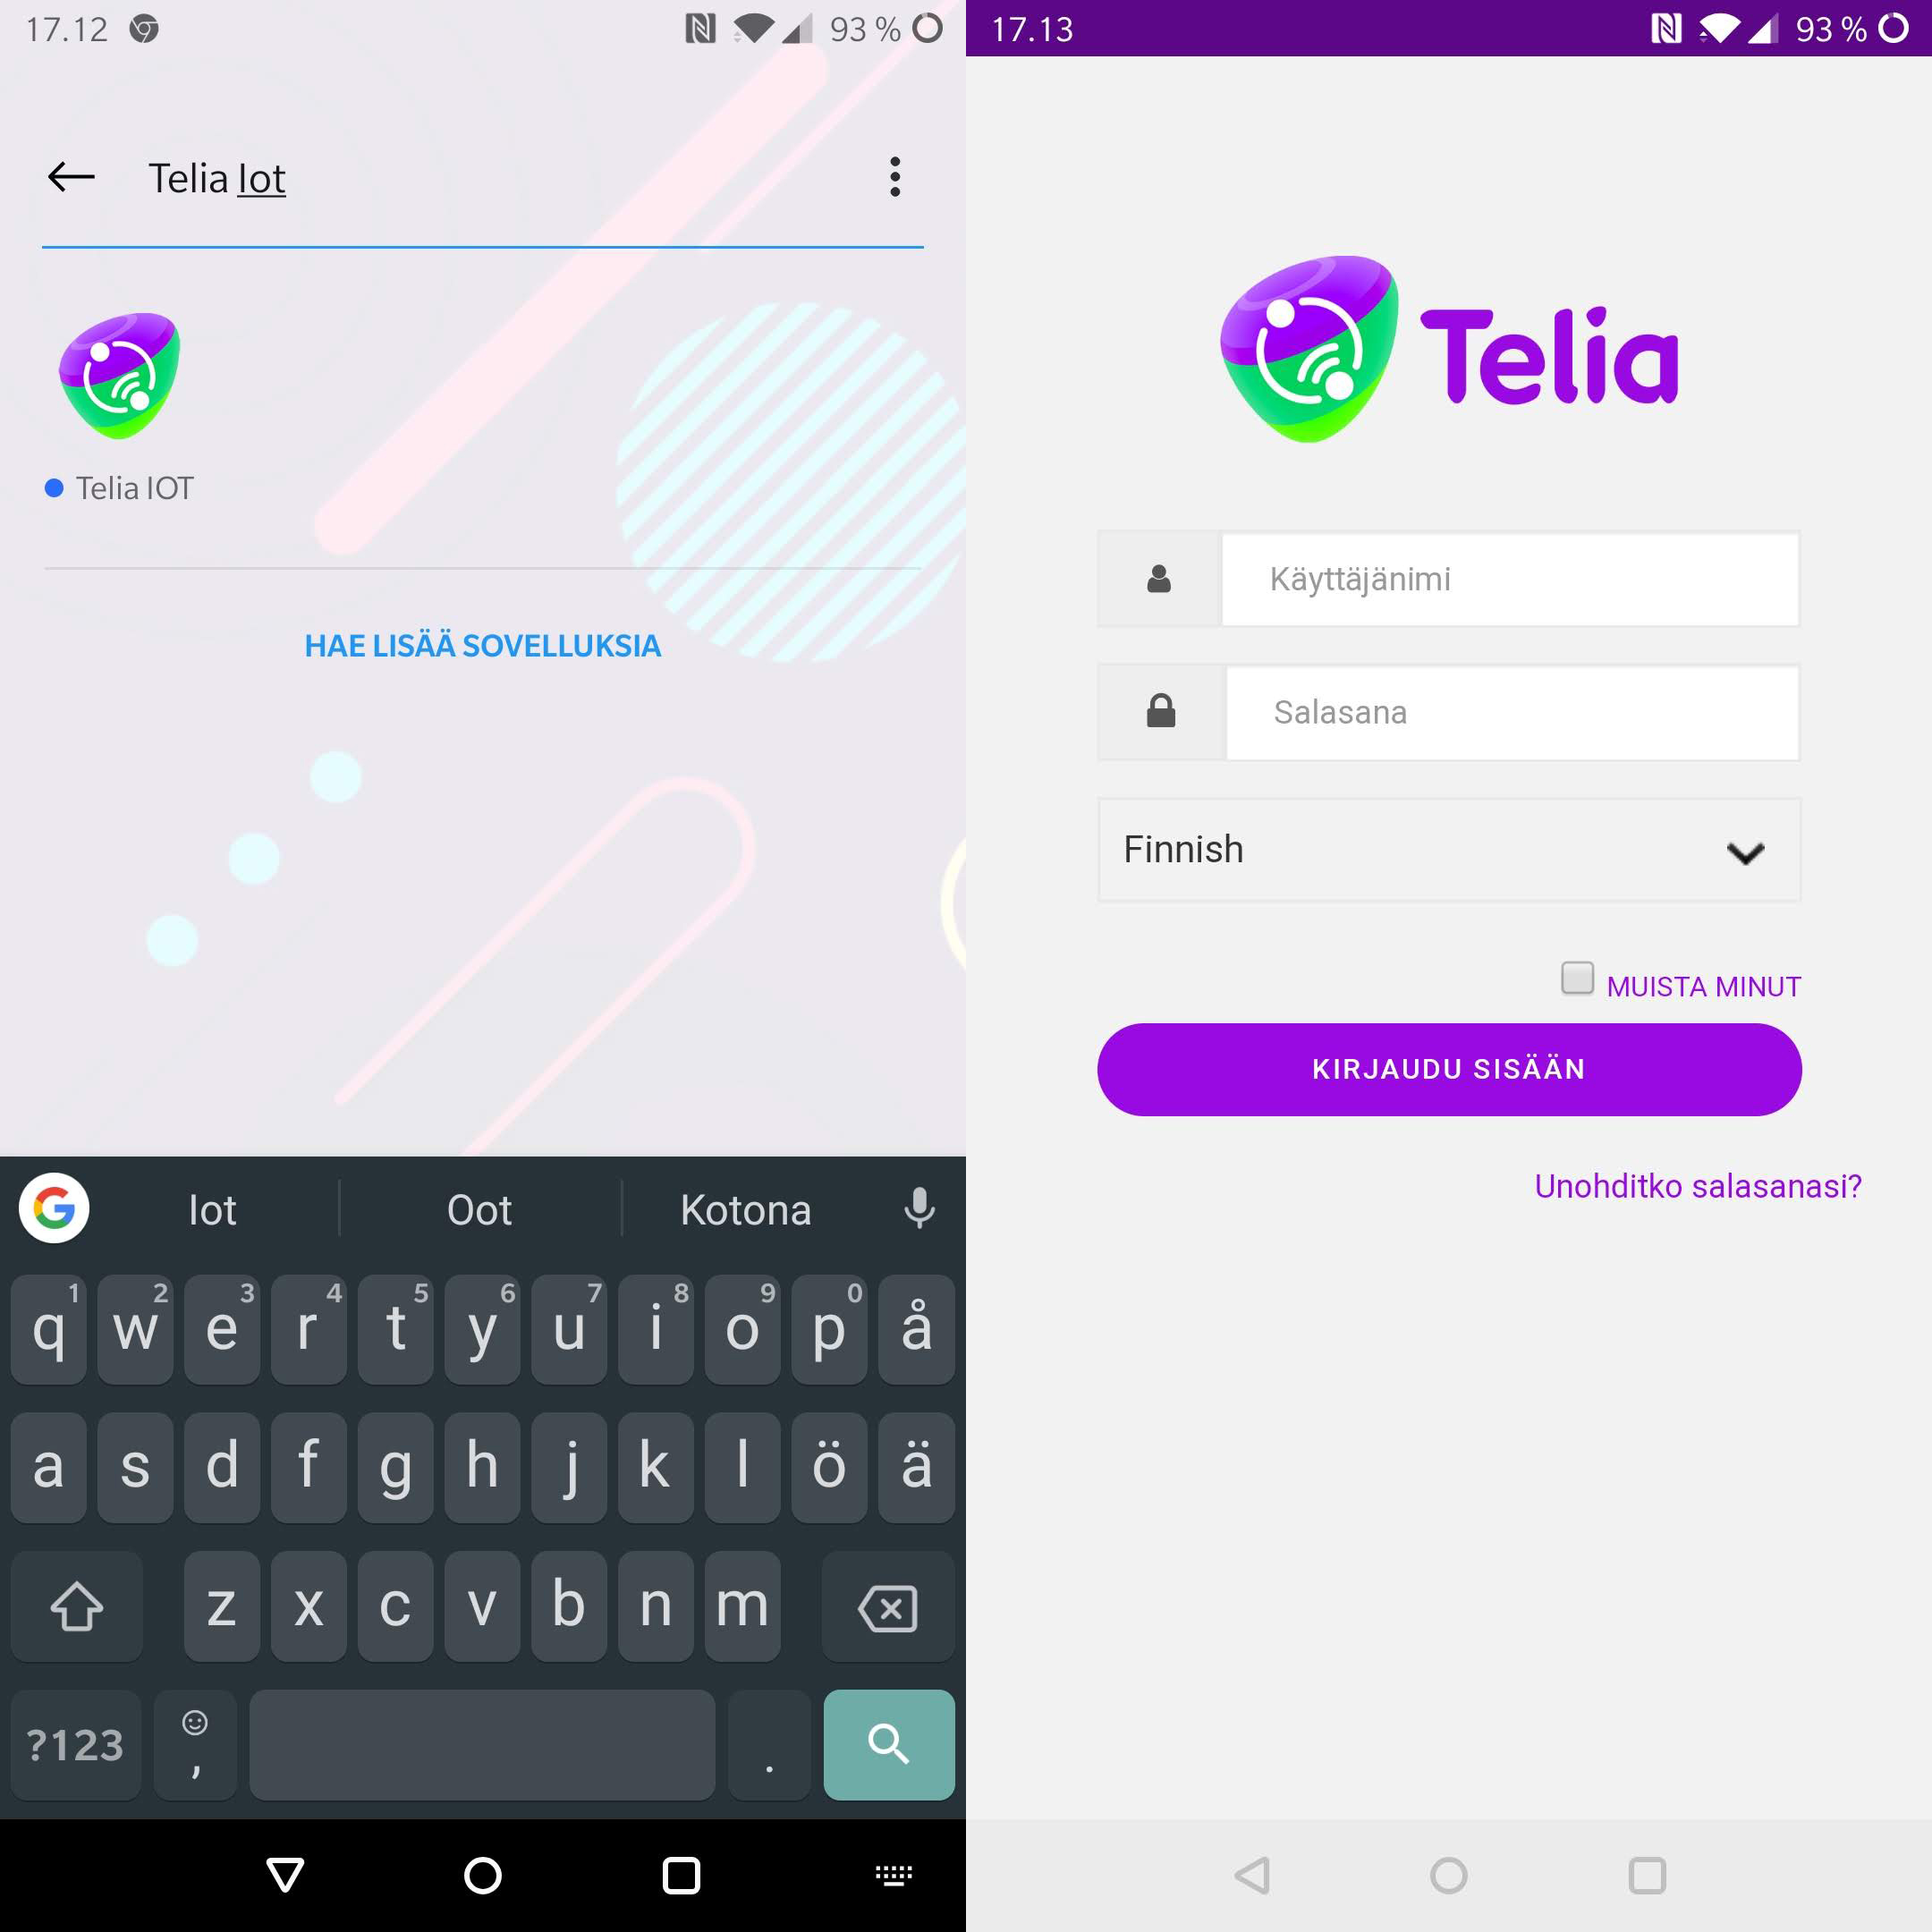
\includegraphics[width=0.9\textwidth]{teliaiot_puhelimessa.jpg}
      \caption{Vasemmalla Telia IoT sovellus asennettuna Android puhelimen sovellusvalikossa. Oikealla sovellus avattuna kokonäytön tilassa.}
      \label{teliaiot_puhelimessa_asennettuna}
\end{figure}

\begin{figure}[!ht]
  \centering
      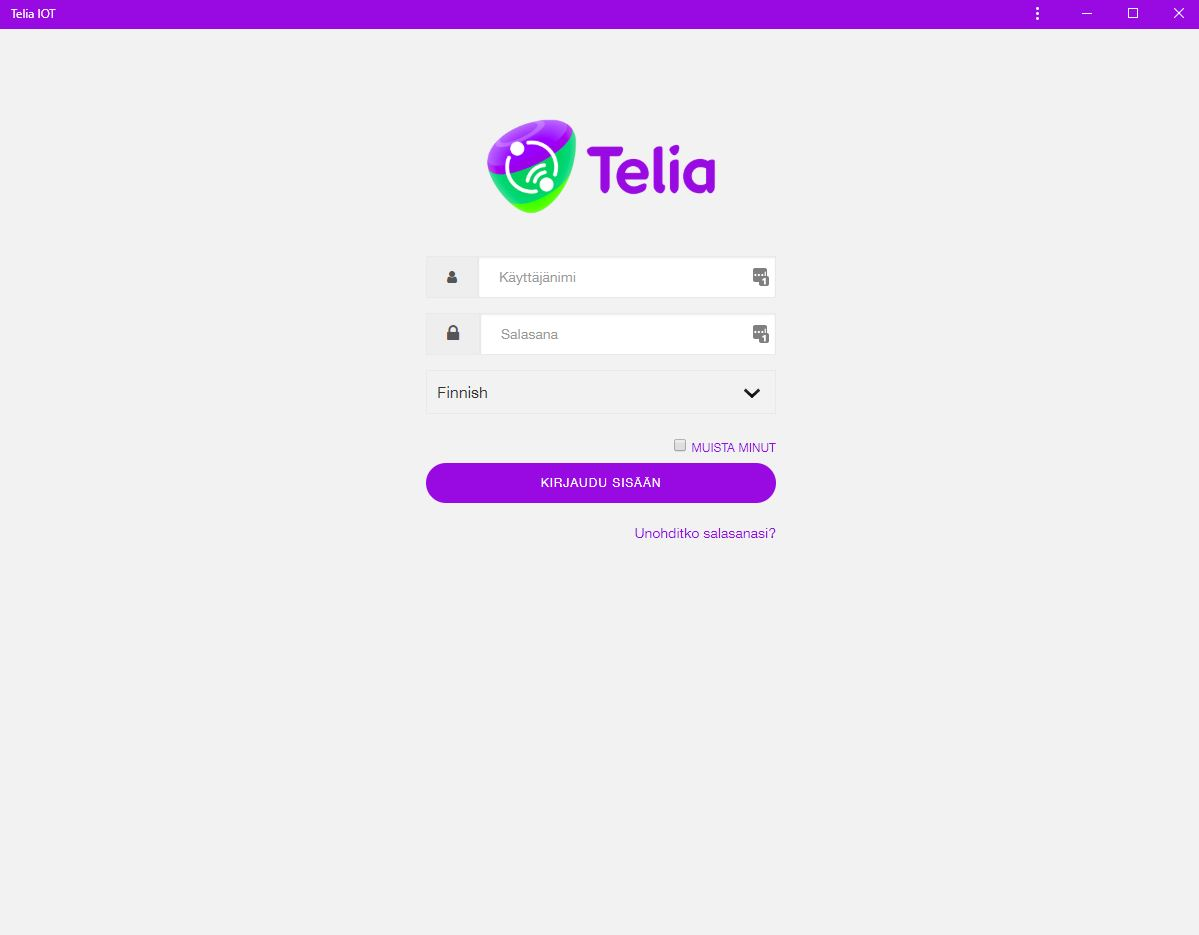
\includegraphics[width=0.9\textwidth]{teliaiot_desktop_installation.jpg}
  \caption{Kuvakaappaus valmiista PWA toteutuksesta TeliaIoT sovelluksesta Windows työasemalla käyttäen Google Chromea.}
  \label{teliaiot_windowsissa_asennettuna}
\end{figure}

\begin{figure}[!ht]
  \centering
      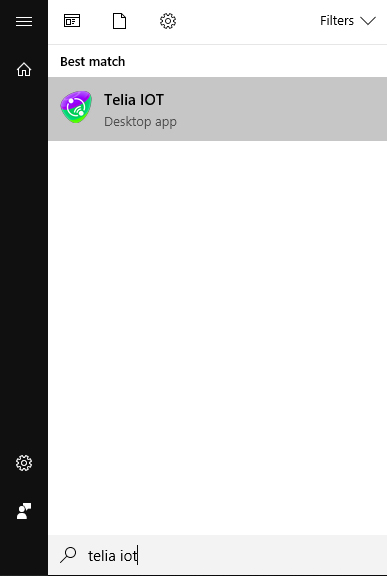
\includegraphics[width=0.9\textwidth]{windows_valikossa.jpg}
  \caption{Telia IoT sovelluskuvake Windows työaseman valikossa asennuksen jälkeen.}
  \label{teliaiot_windowsvalikossa}
\end{figure}



\clearpage
\section{Suorituskyvyn arviointi}

Tässä kappaleessa arvioidaan PWA sovelluksen nopeutta verrattuna normaaliin verkkosivustoon. Mittarina käytetään Googlen Lighthouse työkalua progressiivisuuden ja suorituskyvyn mittaukseen. Lighthousen pisteytys on asteikolla 0-100. Lisäksi otetaan Puppeteer kirjastoa hyödyntäen talteen sovelluksen kääntämiseen kuluva aika, jonka jälkeen sovellus on ensimmäisen kerran valmis vastaanottamaan käyttäjän syötteitä. Mittaukset otetaan Ilman Service Workeria, sekä Service Workerin välimuistin kanssa, jotta saadaan vertailukelpoiset tulokset. Lighthouse suosittelee lisäksi, että sovellusta testataan manuaalisesti useilla eri selaimilla ja alustoilla, jotta käyttökokemuksesta saadaan haluttu \cite{von2018progressive}.

\subsection{Lighthouse pisteet, suorituskyky ja progressiivisuus}

Mikäli sovelluksen Manifest ja Service Worker ovat kunnossa, voidaan Google Chrome selaimen Lighthouse auditointi työkalaulla tarkastella sivun toimintaa ja katsoa täyttääkö se PWA-sovelluksen vaatimukset. Lighthouse on avoimen lähdekoodin työkalu \cite{Google2}, jonka pääasiallinen tarkoitus on parantaa verkkosivujen laatua antamalla pisteytyksen erilaisista kategorioista. Kategorioita ovat: suorituskyky, PWA, hakukoneoptimointi, verkon parhaat käytännöt ja saavutettavuus. Jokaisesta kategoriasta annetaan pisteytys ja joko hylätyt, tai hyväksytyt toimenpiteet. Lighthouse generoi sivustosta raportin. Erityisesti Lighthousen hylättyihin testeihin kannattaa kiinnittää huomiota sovellusta parannettaessa. Jokaisen tarkastuksen (auditoinnin) kohdalla on myös linkki dokumentaatioon miksi kyseinen kohta on tärkeä ja miksi siihen tulisi kiinnittää huomiota. Lisäksi raportissa on mukana erityisesti kehittäjää kiinnostava tieto miten ongelman voi korjata. Lighthousea voi ajaa mitä tahansa nettisivua vasten joko Chrome selaimen kehittäjätyökaluista, komentoriviltä tai node moduulina.

\begin{figure}[h]
\begin{center}
\epsfig{figure=audits_panel.png,  width=0.6\textwidth}
\caption{Kuvakaappaus Google Chrome selaimen kehittäjätyökaluista: Lighthouse työkalun oletus asetukset.}
\label{Lighthouse}
\end{center}
\end{figure}

\clearpage

Sovellusta auditoitiin suoraan tuotantopalvelimelta. Vaihtoehtona olisi ollut auditoida sivua myös kehittäjän koneelta paikallisesta kehitysympäristöstä, mutta tällöin ei olisi saatu oikeita tuloksia loppukäyttäjän näkökulmasta. Esimerkiksi serverin nopeutta ei voida testata, eikä serverin hyödyntämää GZIP pakkausta toimintoa saada auditointiin mukaan lokaalissa ympäristössä. Ensiksi auditoitiin sovelluksen versiota 1.7.0 joka oli kasattu vanhalla Grunt työkalulla, sekä vanhalla Service Worker skriptillä. 

\begin{figure}[h]
\begin{center}
\epsfig{figure=audit1_grunt.png,  width=0.9\textwidth}
\caption{Lighthouse raportti Grunt työkalulla paketoidusta sovelluksesta vanhalla Service Worker skriptillä.}
\label{Lighthouse raportti 1}
\end{center}
\end{figure}

\clearpage

Sovelluksen koko on kasvanut vuosien aikana erittäin laajaksi. Vuoden 2015 lopulla aloitettu projekti ei ole modulaarinen ja sen skriptien lataaminen on selaimessa hidasta. Tästä syystä suorituskykypisteet jäivät hyvin pieniksi. Suorituskykypisteet lasketaan Lightouse työkalun "Time to Interactive" pisteistä, joka tarkoittaa milloin sivu on ensimmäisen kerran käytettävissä ja reagoi käyttäjän toimenpiteisiin. 

Toinen pisteisiin suoraan vaikuttava asia on "First Meaningful Paint", joka tarkoittaa ensimmäistä järkevää näkymää käyttäjälle. Tuloksia analysoimalla saatiin selville, että sovellus täyttää kaikki tarvittavat kriteerit PWA-sovelluksen täyttämiseksi, paitsi suorituskyvyn osalta, jonka takia pistemäärä jäi 73 pisteeseen. PWA-sovelluksille on erittäin tärkeää latautua nopeasti. 


\begin{figure}[!h]
\begin{center}
\epsfig{figure=audit1_webpack.png,  width=0.9\textwidth}
\caption{Lighthouse raportti Webpack työkalulla paketoidusta sovelluksesta uudella Workboxin generoimalla Service Worker skriptillä.}
\label{Lighthouse raportti 2}
\end{center}
\end{figure}

\clearpage

Seuraava auditointi tehtiin Webpackin käännöksellä ja sen hyödyt nähtiin heti. Pelkästään siirtämällä muutama skripti ladattavaksi moduuleina, saatiin sovelluksen lataamista nopeammaksi. Sovelluksen "Time to Interactive" laski yli sekunnin. Myös "First Meaningful Paint" tippui yli 0,5 sekuntia. Web-sovelluksista puhuttaessa on kyse huomattavasta ajasta. Sovelluksen kokonaiskäynnistymisaika on kuitenkin edelleen hidas verrattuna hyvin optimoituihin nykyaikaisiin modulaarisiin sivustoihin. Sekunnin nopeusmuutos antoi kuitenkin täydet 100 pistettä PWA kategoriasta. Sovellus siis täyttää nyt kaikki PWA-sovelluksen kriteerit. Sovelluksen nopeutta mitattiin vielä uudestaan, jotta saataisiin tulokset Service Workerin muodostamasta välimuistin käytöstä.

\begin{figure}[h]
\begin{center}
\epsfig{figure=audit2_webpack.png,  width=0.9\textwidth}
\caption{Lighthouse raportti Service Workerin cachen kanssa.}
\label{Lighthouse raportti 3}
\end{center}
\end{figure}

Toisella kerralla auditoitaessa Lighthousesta täpättiin "Clear storage" valinta pois päältä, jotta sovelluksen välimuistia ei tyhjennettäisi. Sovellus sai toisesta auditoinnista vielä yhden pisteen lisää suorituskykyyn. "First Meaningful Paint" tippui vain 0.1 sekunttia.

\subsection{PWA sivun toistuva avaaminen välimuistista verrattuna ensimmäiseen lataukseen}

Jotta Service Workerin vaikutuksista saataisiin vielä tarkempia tuloksia tehtiin seuraavaksi yksinkertainen toistuva sivulataus sovellukselle. Sovellus avattiin selaimessa ja siitä laskettiin "Dom Interactive" aika. Eli aika, joka selaimelta menee sovelluksen suorittamiseen niin, että selain on ensimmäistä kertaa valmis vastaanottamaan käyttäjän syötteitä ja reagoi toimenpiteisiin. Sovellusta vasten ajettiin yksinkertainen rasitustesti kahdella eri mallilla. Ensimmäisessä mallissa selain käynnistettiin joka kerta uudestaan, jotta selaimen välimuistissa ei olisi aikaisempaa tietoa. Seuraavassa mallissa selainta ei käynnistetty uudestaan ja sivulataus tehtiin kun Service Workerin välimuistiin oli talletettu tietoa. 

Testi suoritettiin käyttämällä Googlen kehittämää Puppeteer kirjastoa. \cite{Google3} Puppeteer on Node kirjasto, joka tarjoaa korkean tason rajapinnan päättömään, eli headless tilassa ajettavaan Chrome, tai Chromium selaimeen kehittäjätyökalu protokollan kautta. Testissä määriteltiin yksinkertaisesti kymmenen ajoa kummallekin tavalle. Selaimen objekteista löytyy performance timing tieto, josta saadaan latenssiin liittyvää suorituskyky tietoa. Testeihin määriteltiin kerättäväksi edellä mainittu "Dom Interactive" aika. Jälkimmäisessä testitapauksessa jossa selainta ei käynnistetty uudestaan testit ajettiin 11 kertaa. Ensimmäistä ajokertaa ei huomioitu, sillä silloin välimuistissa ei vielä ollut mitään tietoa sivusta. Puppeteer aloittaa ajon aina oletuksena tyhjältä pöydältä. Tulokset olivat seuraavat:

\begin{table}[!ht]
\centering
\begin{small}
\caption{Sovelluksen latausajat yksinkertaisessa AB testissä Telia IoT palvelussa. }
\begin{tabular}{|L{3cm}|L{3cm}|L{3cm}|L{3cm}|}
\hline
\textbf{Grunt ei Välimuistia} & 
\textbf{Grunt Välimuistilla} &
\textbf{Webpack ei Välimuistia} &
\textbf{Webpack Välimuistilla}
\\ \hline
544 & 215 &	492 & 183
\\ \hline
501	& 200 & 490 & 189
\\ \hline
479 & 176 & 500 & 189
\\ \hline
491 & 183 & 494 & 181
\\ \hline
491 & 192 & 497 & 179
\\ \hline
492 & 179 &	498 & 182
\\ \hline
487 & 171 &	510 & 180
\\ \hline
482	& 184 &	482 & 179
\\ \hline
500	& 199 &	470 & 182
\\ \hline
475 & 181 &	486 & 184
\\ \hline
  \multicolumn{4}{|c|}{Keskiarvo}
\\ \hline
494,2 &	188 & 491,9 & 182,8
\\ \hline
\end{tabular}
\label{table:latausajatAB}
\end{small}
\end{table}

\clearpage

\begin{figure}[h]
\begin{center}
\epsfig{figure=dominteractive_kaikki.png,  width=0.9\textwidth}
\caption{Dom Interactive kaikki ajat.}
\label{Dom Interactive palkit}
\end{center}
\end{figure}

Testin tulos on selkeä. Service Workerin välimuistista ladattu sivu aukeaa huomattavasti nopeammin kuin ilman Service Workeria. Pyöristettynä Service Workerin välimuistista ladattava sovellus aukeaa 300 millisekuntia nopeammin kuin puhtaalta pöydältä. Eroa Webpackin ja vanhan Grunt työkalun välillä taas ei ollut merkittävästi. Latausaika tuntui vaihtelevan hieman suuntaan tai toiseen. Laskemalla keskiarvo kummastakin ajosta selviää, että Webpackilla tehty ratkaisu oli lopulta hieman nopeampi. Pieni ero Webpackin ja Gruntin välillä johtui siitä, että sovellusta ei oltu optimoitu tarpeeksi modulaariseksi, eikä ylimääräisiä kirjastoja jätetty lataamatta. 

\begin{figure}[!h]
\begin{center}
\epsfig{figure=dominteractive.png,  width=0.7\textwidth}
\caption{Dom Interactive keskiarvoistettu aika.}
\label{Dom Interactive keskiarvoistettu aika}
\end{center}
\end{figure}

Testien perusteella Service Workerin välimuistia hyödyntämällä sovelluksen latausaikaa saadaan siis pienennettyä huomattavasti. 

Sovelluksen latautumista testattiin myös käsin Firefox ja Chrome selaimilla Lighthousen suositusten mukaisesti. Lighthousen kehittäjät suosittelevat myös manuaalista sovellustestausta eri selaimilla ja laitteilla. Sovelluksen latausaika tuntui lähes välittömältä Service Workerin lisäämisen jälkeen. Sekä automaattiset, että manuaaliset testit osoittavat sovelluksen toimivan nopeammin PWA implementaation myötä. 

\begin{figure}[!h]
\begin{center}
\epsfig{figure=google_analytics_teliaiot.png,  width=0.9\textwidth}
\caption{Telia IoT analytiikkaraportti Google Analytics työkalusta.}
\label{Google Analytics raportti Telia IoT}
\end{center}
\end{figure}

Telian tuottamasta analytiikkaraportista selviää vain, että suurin osa käyttäjistä tulee joko Google-Chrome, tai Firefox selaimien kautta. Kyseiset selaimet ovat oletettavasti tarpeeksi uusia tukemaan Service Workeria. Olettama oli, että suurin osa käyttäjistä pystyisi täten käyttämään PWA sovellusta omalla laitteellaan. 

\clearpage

\subsection{Muut PWA sovelluksen mahdolliset mittauskohteet}

Googlen developer dokumentaatiossa tapaustutkimusten osastolla Phil Waltonin artikkelissa \cite{Walton} on mitattu Google Analyticsiä hyödyntäen Googlen omaa I/O web sovelluksen nopeutta tuotannossa oikeilla käyttäjillä. Hyödyntämällä Google Analytics työkalua yhdessä Service Workerin kanssa saadaan vastaus, miten Service Workerin käyttö näkyy loppukäyttäjälle. Pelkästään Lighthouse työkalua hyödyntämällä, tai ajamalla kehittäjän koneella testejä ei saada tarpeeksi kattavia vastauksia. Testien tuloksiin vaikuttaa esimerkiksi se onko käyttäjän Service Worker aktiivinen selaimessa. Mikäli selain on tallettanut useita Service Workereita se sammuttaa niitä tarpeen mukaan. Kun käyttäjä palaa takaisin sivulle jonka Service Worker on jo olemassa, menee sen käynnistymisessä pieni hetki joka taas hetkellisesti nostaa latausaikaa. Chrome Dev Summit konferenssissa oli mitattu Service Workerin käynnistysaikaa sekä tietokoneella, että mobiililaitteella \cite{GoogleDevSummit}. 

\begin{figure}[h]
\begin{center}
\epsfig{figure=sw_bootuptime.png,  width=0.8\textwidth}
\caption{Service Workerin käynnistysaika. Kuvakaappaus \cite{GoogleDevSummit}}
\label{SW bootup time}
\end{center}
\end{figure}

\begin{figure}[h]
\begin{center}
\epsfig{figure=serviceworker_bootuptime.png,  width=0.8\textwidth}
\caption{Service Workerin käynnistysaika millisekunteina eri laitteilla. Kuvakaappaus \cite{GoogleDevSummit}}
\label{SW bootup time on device}
\end{center}
\end{figure}

\clearpage

Konferenssissä esitettyjen lukujen perusteella Service Workerin käynnistysaika on tietokoneella keskimäärin 20-100 millisekuntia ja mobiililaitteella enemmän kuin 100 millisekuntia. Tästä päätellen Service Workerilla on myös muutamia kipupisteitä.

\begin{itemize}
  \item Suorituskyvyn kannalta Service Workerin käynnistysaika ei ole ilmaista. 
  \item Välimuistiluku ei ole aina välitöntä.
  \item Agressiivinen välimuistin käyttö Service Workerissa voi viedä kaistaa pääsivulta. Esimerkiksi jos kaikki sivuston kuvat laitetaan välimuistiin, ne voidaan ladata ennen kuin sovelluksen tärkeämmät tiedot on haettu verkosta.
\end{itemize}

Tarkastellaan Googlen tapaustutkimuksen kautta mittaustuloksia, miten sovelluksen käyttö eroaa loppukäyttäjälle Service Workerin ollessa käytössä. Google asetti Kysymykset seuraavasti.

\textbf{1. Onko Service Workerin välimuisti parempi kuin selaimessa jo oleva HTTP välimuisti?}

Oletus on, että sivustolle uudelleenpalaava käyttäjä saa sivun ladattua nopeammin kuin ensimmäistä kertaa sivustolla vieraileva käyttäjä, sillä selain tallettaa joitain pyyntöjä välimuistiin oletuksena. Service Workerin avulla kehittäjä voi valita mitä tiedostoja sovelluksesta talletetaan. Tutkimuksesta käy ilmi, että Service Workerin välimuistin käyttö on nopeampaa kaikissa eri lähtötilanteissa. Vaikka selaimen välimuistilla päästään ensimmäisessä latauksessa hyvin lähelle samaa lopputulosta on Service Worker silti jonkin verran nopeampi.

\textbf{2. Kuinka paljon Service Workerin käyttö vaikuttaa sivun käytettävyyteen ja latausaikaan?}

Kuinka nopealta sivu tuntuu käyttäjälle, riippumatta oikeasta latausajasta ja perinteisistä latausmetriikoista? Kysymykseen ei ole helppoa vastata ja Walton \cite{Walton} sanookin, että mikään metriikka ei ole täydellinen näin subjektiiviseen kysymykseen. Osa mittauksista on kuitenkin järkevämpiä kuin toiset ja tärkeintä onkin valita oikea metriikka. Lisäksi Walton suositteli aina käyttämään oikeaa sovellusta oikeilla käyttäjillä suorituskyvyn arvioinnissa esimerkiksi hyödyntämällä juuri Google Analytics työkalua yhdessä omien metriikoiden kanssa. Waltonin mielestä lokaalisti ajetut testit eivät ole oikeastaan koskaan tarpeeksi kattavia.

Waltonin tapaustutkimuksessa \cite{Walton} mitattiin sivuston latausaikaa, joka on hyvä mittaus ensimmäiseen kysymykseen, samaan tapaan kuin Lighthousen auditointi sivuston piirtämiseksi. Se ei kuitenkaan vastaa toiseen kysymykseen. Huomioidaan vielä, että sivuston latausaika ei ole sama asia kuin milloin käyttäjä voi alkaa käyttämään sovellusta. Kaksi sovellusta täysin samalla latausajalla voi tuntua täysin erilaiselta. Esimerkiksi sovellus joka näyttää aloitusruudun, tai latausindikaattorin voi tuntua käyttäjästä huomattavasti nopeammalta kuin sovellus joka näyttää vain tyhjää sivua muutaman sekunnin. Waltonin esimerkissä metriikaksi valittiin kulunut aika ensimmäiselle piirrolle. Tämä mittaus on tärkeä, sillä se määrittelee ensikokemuksen käyttäjälle. Hyvä ensikokemus voi vaikuttaa positiivisesti sovelluksen loppukäyttöön. 

Latausajan mittaukset jaettiin tapaustutkimuksessa kolmeen eri kategoriaan.

\begin{itemize}
  \item \textbf{Controlled:} Service Worker määrittelee välimuistiin talletettavat asiat ja sovellusta voi käyttää Offline tilassa.
  \item \textbf{Supported:} Service Worker on tuettuna selaimessa, mutta se ei ole vielä tallettanut mitään. Kyseessä on ensimmäistä kertaa sivustolla vieraileva käyttäjä.
  \item \textbf{Unsupported:} Käyttäjä jonka selain ei tue Service Workeria ollenkaan. 
\end{itemize}

\begin{figure}[h]
\begin{center}
\epsfig{figure=google_case_study_1.png,  width=1.0\textwidth}
\caption{Keskimääräiset latausajat Googlen IOWA sovelluksessa. Kuvakaappaus Google Developer portaalista.}
\label{Google AVG load times}
\end{center}
\end{figure}

Kuvaajasta \ref{Google AVG load times} nähdään, että Service Workerin hallitsema välimuisti (sininen pylväs) lataa sivut nopeammin kuin käyttäjillä, joilla on selaimen välimuistissa jo tietoa (punainen pylväs). Mielenkiintoista on myös huomata, että mobiilikäyttäjillä latausaika on Service Workerin ollessa käytössä lyhyempi, kuin uusilla tietokone käyttäjillä. 

\begin{table}[h]
\centering
\begin{small}
\caption{Keskimääräinen sivuston lataamisaika tietokoneella IOWA tapaustutkimuksessa \cite{Walton} }
\begin{tabular}{|L{5cm}|L{5cm}|L{5cm}|}
\hline
\textbf{Service Workerin tila} & 
\textbf{Käyttäjätyyppi} &
\textbf{Keskimääräinen latausaika (ms)}
\\ \hline
Käytössä & 
Palaava käyttäjä &
2568
\\ \hline
Tuettu, ei käytössä & 
Palaava käyttäjä &
3612
\\ \hline
Tuettu, ei käytössä & 
Uusi käyttäjä &
4664
\\ \hline
\end{tabular}
\label{table:loading time on pc}
\end{small}
\end{table}

\clearpage

\begin{table}[h]
\centering
\begin{small}
\caption{Keskimääräinen sivuston lataamisaika mobiililaitteella IOWA tapaustutkimuksessa \cite{Walton} }
\begin{tabular}{|L{5cm}|L{5cm}|L{5cm}|}
\hline
\textbf{Service Workerin tila} & 
\textbf{Käyttäjätyyppi} &
\textbf{Keskimääräinen latausaika (ms)}
\\ \hline
Käytössä & 
Palaava käyttäjä &
3760
\\ \hline
Tuettu, ei käytössä & 
Palaava käyttäjä &
4843
\\ \hline
Tuettu, ei käytössä & 
Uusi käyttäjä &
6158
\\ \hline
\end{tabular}
\label{table:loading time on mobile}
\end{small}
\end{table}


Taulukoiden latausajoista nähdään, että ero Service Workerin ollessa päällä mobiililaitteella ja verrattuna uuteen työasema vierailijaan on noin sekunnin nopeampaa mobiililaitteella. Vastatakseen toiseen kysymykseen, kuinka paljon Service Worker vaikuttaa sovelluksen käytettävyyteen, Googlen tapaustutkimuksessa otettiin mittaukset "Ensimmäinen piirto" osiosta.

\begin{figure}[!h]
\begin{center}
\epsfig{figure=google_case_study_2.png,  width=0.7\textwidth}
\caption{Keskimääräiset ensimmäisen piirron ajat Googlen IOWA sovelluksessa. Kuvakaappaus Google Developer portaalista.}
\label{Google AVG load times 1}
\end{center}
\end{figure}

Kuvasta \ref{Google AVG load times 1} käy ilmi, että Service Workerilla on paljon pienempi vaikutus "Ensimmäinen piirto" kohdassa mobiililaitteella. Dataa täytyy kuitenkin vielä tarkastella lisää, jotta saadaan käsitys miksi asia on näin. "Ensimmäinen piirto" tuloksista on poimittu joka ikinen sivulataus ja muodostettu seuraava kuvaaja.

\begin{figure}[h]
\begin{center}
\epsfig{figure=google_case_study_3.png,  width=0.9\textwidth}
\caption{Ensimmäinen piirto Service Workerilla ja ilman (Tietokone). Kuvakaappaus Google Developer portaalista.}
\label{Google AVG load times 2}
\end{center}
\end{figure}

Kuvasta \ref{Google AVG load times 2} huomataan, että Service Workerin ollessa käytössä ensimmäinen piirtoaika on pienentynyt noin puoli sekuntia. Lisäksi Service Workerin ollessa käytössä saatiin "ensimmäinen piirto" melkein heti työasema käytössä. Mielenkiintoista kuvan graafissa on se, että Service Workerin ollessa käytössä on jakauma kellon muotoinen, eikä laskeva. Waltonin tutkittua asiaa selvisi että jakauma johtuu siitä että Service Worker ei ole aina aktiivinen selaimessa. Selain lopettaa Service Worker threadin ajamisen säästääkseen resursseja. Jokaista Service Workeria ei olisikaan järkevää pitää aktiivisena jos olisi vieraillut sadoilla eri verkkosivuilla. Tämä selittää jakauman. Joillakin käyttäjillä Service Worker on saattanut olla sammunut ja sen uudelleen käynnistämisessä on kestänyt pieni hetki. Kuvasta  nähdään myös, että vaikka Service Worker olisi sammuksissa, saadaan sen avulla ladattua sivusto nopeammin, kuin että selain tekisi kaikki kyselyt puhtaasti verkosta. 

\clearpage

\begin{figure}[h]
\begin{center}
\epsfig{figure=google_case_study_4.png,  width=0.9\textwidth}
\caption{Ensimmäinen piirto Service Workerilla ja ilman (Mobiililaite). Kuvakaappaus Google Developer portaalista.}
\label{Google AVG load times 3}
\end{center}
\end{figure}

Mobiililaitteella Kuvan käyrä on melko pitkä ja eroaa huomattavasti tietokoneesta. Tämä johtuu luultavasti siitä, että mobiililaitteella Service Worker skriptin uudelleenkäynnistys kestää luonnollisesti kauemmin kuin tietokoneella. Tämä antaa selityksen myös kaaviossa \ref{Google AVG load times 3} näkyvään pieneen "Ensimmäinen piirto" eroon. Tämä myös todistaa sen että testit on järkevää suorittaa oikeilla käyttäjillä oikeassa palvelussa sillä näin kaikki käyttötapaukset tulee otettua huomioon. Oikeilla käyttäjillä saadaan huomioitua tilanne jossa Service Worker on ollut esimerkiksi sammuksissa, tai että välimuistin tilanne on ollut eri kuin lokaaleissa koetilanteissa.

\begin{table}[h]
\centering
\begin{small}
\caption{Mediaani ensimmäiselle piirrolle (ms) }
\begin{tabular}{|L{5cm}|L{5cm}|L{5cm}|}
\hline
\textbf{Service Workerin tila} & 
\textbf{Tietokone} &
\textbf{Mobiililaite}
\\ \hline
Käytössä & 
583 &
1634
\\ \hline
Tuettu, ei käytössä &
912 &
1933
\\ \hline
\end{tabular}
\label{table:median first paint}
\end{small}
\end{table}

Taulukosta \ref{table:median first paint} nähdään mikä vaikutus Service Workerilla on sovelluksen nopeuteen. Nopeus taas vaikuttaa suoraan sovelluksen käyttökokemukseen. Niin tietokoneella, kuin mobiililaitteella sovelluksen latausaika on lyhyempi, mikäli Service Worker on käytössä ja ladannut välimuistiin tietoa. Kun Service Workerista ladataan tietoa, laitteen ei tarvitse myöskään kuluttaa virtaa verkkopyyntöihin \cite{8456349}. Kyseisen artikkelin mukaan Service Workerin käyttö säästi noin 25\% dataliikenteestä ja antoi myös offline tuen sovelluksille. Service Workerin käyttö kuitenkin kuluttaa enemmän virtaa laitteesta \cite{malavolta2017assessing}. Vaikka verkkoliikenne pienenee, käyttää Service Worker enemmän virtaa laitteesta. Työssä tutkittiin 28 erilaista tapausta. 7 eri PWA sovellusta, kaksi eri laitetta ja kaksi eri verkkoa. Wifi ja 2G. 20 tapauksessa Service Workerin käyttö PWA sovelluksessa lisäsi laitteen virrankulutusta. 8 tapauksessa virrankulutus oli kuitenkin pienempää. Työn tulos indikoi, että kehittäjän tulee  olla varovainen teknologiaa hyödyntäessä. Useimmiten virrankäytön lisääminen on kuitenkin järkevää käyttökokemuksen kannalta, sillä virrankulutuksen lisääntyminen oli hyvin pientä verrattuna sivustoon joka ei käyttänyt Service Workeria.


\clearpage
\section{Pohdinta}

PWA:n käyttöönotossa esiintyi muutamia ongelmia projektin aikana. Projektin työkalut olivat vanhentuneet, joten ensimmäinen varsinainen ongelma oli yhteensopivuusongelma Service Worker työkalun käytössä. Työkalujen kanssa tehtiin jonkin verran töitä, jotta ne saatiin pelaamaan yhteen. Toinen kehityksen aikana ilmennyt ongelma oli sovelluksen näyttäytyminen välimuistista kun Service Worker oli saatu käyttöön. Google Chromen kehittäjäkonsolissa on Service Worker välilehdellä täpät “update on reload“ ja “Bypass for network“ jotka ruksattiin käyttöön. Näin kehittäjä näkee aina uusimmat muutokset selaimessaan. Muutoin koodiin tehdyillä muutoksilla ei välttämättä olisi vaikutusta, sillä Service Worker näyttäisi tiedostoja ja koodia välimuistista. 

"Bypass for network" täpän käytöstä aiheutui kuitenkin se, että kehityksen aikana ei voitu hyödyntää Service Workerin välimuistia kun välimuistin käyttö ohitettiin. Service Workerin tuomaa nopeutta ei siis saatu hyödynnettyä kehityksen aikana.

Kolmas haaste liittyi sovelluksen modulaarisuuden puuttumiseen. Nykyisessä sovelluksessa on paljon koodia jota ei ajeta ohjelman käynnistyessä. Tästä syystä Lighthousen auditointityökalu antoi huonot suorituskykypisteet sovellukselle. Koodien pakkaamiseen tehtiin joitakin muutoksia työkalujen käyttömahdollisuuksien mukaan ja tilannetta saatiin hieman parannettua. Myös tietokantakyselyitä koitettiin vähentää. Kyselyiden vähentäminen on kuitenkin haastavaa palvelussa, joka perustuu reaaliaikaiseen dataan. Tästä syystä sovelluksen suorituskykypisteet jäivät mitättömiksi Lighthouse mittauksissa. 

Puppeteer mittauksista saatiin raakaa numerodataa Service Workerin käytöstä. Testit osoittavat selvästi että välimuistin käyttö nopeuttaa sovelluksen toimintaa. Puppeteer testeissä ei kuitenkaan käynyt ilmi kaikki reaalimaailman tapaukset. Esimerkiksi tilanne jossa Service Worker on sammunut selaimessa. Selain siis saattaa sammuttaa Service Workereita jos sivustolla ei ole vierailtu vähään aikaan ja Workereita on kertynyt useampia. Tällöin Service Workerin käynnistämisestä seuraa pieni latenssi, joka vaikuttaa suoraan sivuston latausaikaan. Googlen tapaustutkimuksessa on kuitenkin laskettu että Service Workerin käynnistymisaika on vähintään 100 millisekuntia mobiili laitteilla ja tietokoneilla 20-100 millisekuntia. Service Workerin käyttö ei siis ole ilmaista. Tästä huolimatta kaikki sivulataukset olivat nopeampia Googlen tapaustutkimuksessa jos Service Worker oli käytössä ja vaikka se olisi sammunut. Googlen tapaustutkimuksessa myös vertailtiin selaimen omaa välimuistin käyttöä Service Workeriin. Jokaisessa tapauksessa Service Worker oli nopeampi. 

Googlen tapaustutkimuksessa tehtiin myös muita laajempia mittauksia mitä ei keretty Telia IoT projektissa tekemään. Tapaustutkimuksessa hyödynnettiin Google Analyticsiä laajemmin ja käyttäjistä kerättiin muun muassa seuraavaa tietoa. 

\begin{itemize}
  \item Offline käyttöä havaitiin noin 5\% käyttäjistä. Offline käytöksi laskettiin vähintään yksi toimenpide ilman verkkoyhteyttä.
  \item Sovellusilmoitukset salli melkein 60\% käyttäjistä. 36\% Ei asettanut oikeuksia ja noin 5\% esti sovellusilmoitusten näyttämisen. Tutkimus vähintäänkin osoittaa, että mikäli sovelluks koetaan hyödylliseksi ihmiset pääosin sallivat sovellusilmoitukset. 
  \item Sovelluksen asennusbannerista otettiin ylös tiedot pikakuvakkeen lisäämisestä työpöydälle. 11,5\% käyttäjistä loi uuden pikakuvakkeen. 26\% hylkäsi ilmoituksen ja 62,4\% käyttäjistä jätti koko ilmoituksen huomiotta.
\end{itemize}
 
Service Workerin selkeä kipupiste on välimuistin hallinta. Kehittäjän tulee miettiä tarkkaan mitä tietoa kannattaa ja voi laittaa välimuistiin. Kaikkia verkkokaupan kuvia ei esimerkiksi ole järkevää laittaa välimuistiin. Huolellisella välimuistisuunnittelulla ja käyttämällä Service Workerin kanssa erilaisia strategioita saadaan aikaan järkevä kokonaisuus. Koska tallennustila on rajallinen, esimerkiksi mobiililaitteita varten nyrkkisääntönä voidaan varata noin 50 megatavua tilaa välimuistille. \cite{Love}

Itse PWA:n luominen olemassa olevaan sovellukseen on loppujen lopuksi yksinkertainen prosessi. Sovelluksen tarvitsee ainoastaan rekisteröidä Service Worker ilman että se edes tekisi mitään. Lisäksi tarvitaan yksinkertainen JSON manifesti, jossa on määritelty sovelluksen nimi, ikoni ja muut tarvittavat tiedot. Tiedostoja pystyy jopa generoimaan netissä jos sellaista ei halua kirjoittaa itse. Lisäksi tarvitaan sovelluksen ikoni ja sovellus tulee tarjoilla HTTPS protokollan ylitse. Mitä tulee HTTPS protokollaan se on yleensä palvelinta hallitsevan henkilön huoli. HTTPS sertifikaatteja voi myös nykyisin hankkia itse ilmaiseksi Let's Encrypt varmentajalta joka on ilmainen, avoin ja automatisoitu palvelu.

Service Workerin tuomat hyödyt ovat siis selkeät ilman huomattavia panostuksia sovelluskehityksessä ajallisesti tai rahallisesti. Mikäli sovelluksesta halutaan  mobiiliversio, eikä ole tarvetta julkaista tuotetta Applen tai Googlen mobiilikaupoissa, eikä ole tarvetta käyttää mobiililaitteen natiiveja rajapintoja joihin selaimella ei pääse käsiksi, voidaan hyvin käyttää PWA-sovellusta. PWA-sovelluksen toteuttaminen automatisoiduilla työkaluilla on nopeaa ja edullista. Service Worker nopeuttaa sovelluksen latausaikaa mikäli välimuististrategia on mietitty ja toteutettu oikein. 

Ainoa yllättävä tutkimustulos PWA sovelluksista oli kasvanut virrankulutus. Alkuperäinen oletus oli että virrankulutus tippuisi PWA sovelluksissa jonkun verran kun verkkokyselyitä ei tarvitse tehdä niin paljoa. Varsinaista selitystä virrankulutuksen kasvulle ei kuitenkaan löytynyt. 

Tämän tutkimuksen ja Googlen tapaustutkimuksen lopputuloksena:

\begin{itemize}
  \item Sivut latautuivat keskimäärin huomattavasti nopeammin Service Workerin ollessa käytössä jos sen välimuistissa oli jo jotain.
  \item Vierailut sivuille jotka Service Worker oli jo ladannut välimuistiin aukesivat melkein heti.
  \item Googlen tutkimuksessa huomattiin että mikäli Service Worker on sammuneena selaimessa, kestää sillä pieni hetki käynnistyä. Tästä huolimatta sivusto jolla Service Worker oli käytössä ja sammuneena latautui silti nopeammin kuin sivu jolla ei ollut ollenkaan Service Workeria.
  \item Mobiililaitteilla Service Workerin käynnistyminen kestää kauemmin kuin tietokoneella.
\end{itemize}

Huomioon otettavaa on myös, että mikäli Service Workerin ja PWA sovelluksen suorituskykyä halutaan mitata, tulee suunnitella jokaista sovellusta varten oma mittaus strategia. Minkälaisia arvoja ja mittapisteitä halutaan ottaa huomioon? Jos esimerkiksi mittapisteenä halutaan käyttää "ensimmäinen piirto" arvoa, tulee huomioida ensimmäinen järkevä renderöinti. Joissain tapauksissa selain saattaa ilmoittaa ensimmäisen piirron arvon tyhjälle sivulle. Sivu voi olla tyhjä, riippuen tyylien ja sisällön lataustavasta. Tärkeää on tässä tapauksessa määritellä mikä on ensimmäinen järkeenkäypä näkymä sivulla.  

Lopputulemana Telia IoT projektissa saatiin sovelluksesta toteutettua 100\% PWA sovellus Googlen Lighthouse työkalun pisteytyksen mukaan. Sovellus oli mahdollista asentaa puhelimeen ja sovellus tarjosi asennusikkunan sivustolla vierailtaessa. Service Workerin välimuistiin oli määritetty tallennettavaksi kaikki sovelluksen skriptit, kuvat ja näkymät etukäteen. Service Worker siis nopeutti sovelluksen näkymien lataamista huomattavasti. Lisäksi olisi ollut mahdollista lähettää myös sovellusilmoituksia, mutta siihen ei ollut tarvetta. Sovellusta ei voi käyttää offline tilassa, sillä suurin osa näkymistä perustuu reaaliaikaiseen tietoon. Vanhaa dataa olisi ollut kyllä  mahdollista hakea ja tallettaa, mutta sitä ei ehditty toteuttamaan. Offline näkymäksi asetettiin vain viesti: "sovellusta ei voi käyttää offline tilassa". Mahdollisuutena offline käytössä olisi ollut tallettaa datakutsuja Service Workeriin ja näyttää offline tilassa vanhoja mittapisteitä ilmanlaadusta. Tätä ei myöskään toteutettu.

Useat yritykset ovat alkaneet huomata PWA sovelluksen hyötyjä. Nopeat ja natiivin kaltaiset palvelut sitouttavat käyttäjiä tehokkaammin kuin hitaat ja kömpelöt sovellukset. PWA sovelluksen turvallisuus HTTPS protokollan ylitse yhdessä nopeuden kanssa ovat sen kaltaisia muuttujia, että PWA sovellukset eivät tule katoamaan lähitulevaisuudessa. \cite{8441701} 

PWA sovelluskehitys myös mahdollistaa saman kehittäjän käyttämisen kaikille laitealustoille mikä on kustannustehokkaampaa ja time-to-market aikaa saadaan pienennettyä. PWA sovellus pitää siis sisällään parhaat puolet natiiveista sovelluksista ja normaaleista verkkosovelluksista. 

Yksi mielenkiintoinen seikka PWA maailmassa on artikkelissa \cite{8287006} mainitut älytelevisiot. Älytelevisioiden sovelluskehitys on hyvin pirstoutunutta tällä hetkellä. Jokaisella laitevalmistajalla on oma käyttöliittymä ja ohjelmistokehys. Lisäksi televisioita voidaan laajentaa erilaisilla lisävarusteilla, kuten Apple TV tai Chromecast tyyppisillä streaming laitteilla. Lähes jokaisessa modernissa televisiossa on kuitenkin verkkoselain. PWA voisi olla yksi ratkaisu televisioiden parissa. Jokaiselle televisiolle voitaisiin järkevästi kehittää sovelluksia hyödyntämällä selainta. 

Teknologian idea ei päde pelkästään televisioihin. Samalla tavalla PWA-sovelluksia voisi hyödyntää autoissa, tai muissa kodin esineiden internet tyyppisissä laitteissa. Yhteistyö laitevalmistajien kesken olisi tärkeää, sillä mikään ekosysteemi tai yritys ei voi tehdä kaikkea itse. Myös käyttöliittymät ja käyttökokemus kulkevat käsi kädessä suorituskyvyn ja laitealustojen kanssa. PWA:n käyttömahdollisuudet ovat tulevaisuudessa lähes rajattomat, mikäli laitevalmistajat ja yritykset ymmärtävät tehdä yhteistyötä ja omaksua uuden teknologian. 

% yksi näistä tai ...
%\bibliographystyle{plain}
%\bibliographystyle{acm}
\bibliographystyle{ieeetr}

% ... tai tämä 
%\bibliographystyle{apalike}

\clearpage
\bibliography{lahteet}

\lastpage

\appendices

\end{document}
